\chapter{Theory}

\lettrine[lines=4, loversize=-0.1, lraise=0.1]{T}{he Jam is here}, but nowhere to be found.

\section{Single Target State Estimation}\label{sec:STT}

Single target state estimation concerns with the problem of estimating the state of a known target under uncertainty. There is uncertainty in how the state evolves over time, as well as uncertainty in how accurate sensor readings of the target are. In order to model and deal with uncertainty, a probabilistic framework is employed. By using a probabilistic framework, the single target tracking problem can be expressed in the following way. 

\begin{equation}
    \begin{split}
        x_{k} &= f_{k-1}(x_{k-1},v_{k-1}) \\
        y_{k} &= h_k(x_k,w_k) 
    \end{split}\label{eq:mm}
\end{equation}

The state, $x_k$, of a known target is assumed to evolve over time according to a discrete time Markov model $f(\cdot)$ and is subject to motion noise $v_k$. Each incremental time step is denoted by $k$. The initial state is distributed according to $x_0 \sim p(x_0)$. At each time step a measurement, denoted $y_k$, is generated as a function $h(\cdot)$ of the state $x_k$ and the measurement noise $w_k$.

The optimal filtering problem is to compute the posterior density $p(x_k|y_{1:k})$ when $ k \geq 1, k \in \mathbb{N}$. By using Bayesian statistics, the state conditioned on all measurements up to time $k$ can be expressed as

\begin{equation}
    \begin{split}
        p(x_k|y_{1:k}) &= \int p(x_{0:k}|y_{1:k})dx_{0:k-1}
    \end{split}\label{eq:rec1}
\end{equation}

\begin{equation}
    \begin{split}
        p(x_{0:k}|y_{1:k}) &= \frac{p(y_{1:k}|x_{0:k})p(x_{0:k})}{p(y_{1:k})}
        \propto p(x_0)\prod\limits_{i=1}^{k}p(y_i|x_i)p(x_i|x_{i-1})
    \end{split}\label{eq:rec2}
\end{equation}

A drawback with the formulation in \eqref{eq:rec1}-\eqref{eq:rec2} is that complexity grows with $k$. Instead, it is possible to express the posterior density as a recursive solution which utilises the previous posterior density. The recursive solution is expressed in two steps, the prediction step and the update step. The prediction step represents the expected posterior density at time $k$ conditioned on all measurements up to time $k-1$, which can be expressed using the Chapman-Kolomogrov equation as \todo{reference} 

\begin{equation}
    \begin{split}
        p(x_k|y_{1:k-1}) &= \int p(x_k|x_{k-1})p(x_{k-1}|y_{1:k-1})dx_{k-1}
    \end{split}\label{eq:pred}
\end{equation}

The update step incorporates knowledge from the measurement $y_k$ into the prediction step, yielding the updated posterior as

\begin{equation}
    \begin{split}
        p(x_k|y_{1:k}) &= \frac{p(y_k|x_k)p(x_k|y_{1:k-1})}{p(y_k|y_{1:k-1})}
    \end{split}\label{eq:update}
\end{equation}

The two equations \eqref{eq:pred} and \eqref{eq:update} present a general recursive solution to the optimal filtering problem. However, they do not offer a general closed form solution, which makes them difficult to implement in practice. However, under certain conditions closed form solutions can be found, such as the Kalman Filter. 

\subsection{Kalman Filter}
The Kalman Filter (KF) offers a closed form solution to the recursive optimal filtering formulation found in \eqref{eq:pred}-\eqref{eq:update} by imposing the following conditions

\begin{itemize}
    \item Both the state and measurement evolve over time according to a linear model.
    \item The underlying prior distribution $p(x_0)$ is assumed to be Gaussian, i.e. $x_0 \sim \mathcal{N}(\hat{x}_0,P_0)$.
    \item Motion noise $v_k$ and measurement noise $w_k$ are i.i.d. Gaussian.
\end{itemize}

With these conditions the general motion and measurement model equations \eqref{eq:mm} can be rewritten as

\begin{equation}
    \begin{split}
     x_k &= F_{k-1}x_{k-1} + v_{k-1}, \quad v_k \sim \mathcal{N}(0,Q_{k-1}) \\
     y_k &= H_kx_k + w_ k, \quad\quad\enspace\enspace w_k \sim \mathcal{N}(0,R_{k})
    \end{split}\label{eq:motion_meas}
\end{equation}

(We impose that both motion and sensor noise are zero-mean is to keep subsequent equations more clear). Since all densities are of Gaussian nature, only two moments are needed to describe the posterior density: the mean $\hat{x}_{k|k}$ and the covariance $P_{k|k}$. As such, key densities in the recursive formulation \eqref{eq:pred} and \eqref{eq:update} can be expressed as

\begin{equation}
        p(x_{k-1}|y_{1:k-1}) \sim \mathcal{N}(\hat{x}_{k-1|k-1}, P_{k-1|k-1})
\end{equation}
\begin{equation}
        p(x_{k}|y_{1:k-1})   \sim \mathcal{N}(\hat{x}_{k|k-1}, P_{k|k-1})
        \label{eq:kfpred}
\end{equation}
\begin{equation}
        p(x_{k}|y_{1:k})     \sim \mathcal{N}(\hat{x}_{k|k}, P_{k|k}) 
        \label{eq:kfupdate}
\end{equation}

The prediction step in the KF corresponds to finding expressions for the moments found in \eqref{eq:kfpred}. Since the models are linear, this corresponds to finding the expected value and covariance of a linearly scaled and shifted Gaussian density.

\begin{equation}
    \begin{split}
        \mathbb{E}[x_k|y_{1:k-1}] \equiv \hat{x}_{k|k-1} &= F_{k-1}\hat{x}_{k-1|k-1} \\
        \text{Cov}[x_k|y_{1:k-1}] \equiv P_{k|k-1} &= F_{k-1}P_{k-1|k-1}F_{k-1}^{T} + Q_k 
    \end{split}
\end{equation}

The update step in the KF is divided into several components which are used to find expressions for the moments of the posterior density. Detailed information on how these components are derived can be found in XX\todo{reference}. 

\begin{align}
    \begin{split}
        v_k &= y_k - H_k\hat{x}_{k|k-1}
    \end{split}\label{eq:innovation} \\
    \begin{split}
        S_k &= H_{k}P_{k|k-1}H_{k}^{T} + R_k
    \end{split}\label{eq:sk} \\
    \begin{split}
        K_k &= P_{k|k-1}H_{k}^{T}(S_k)^{-1}
    \end{split}\label{eq:kalmangain}
\end{align}

The term $v_k$ in \eqref{eq:innovation} is the so called \textit{innovation} and represents the difference between the actual measurement and the predicted measurement. The innovation is zero-mean and has a covariance equal to $S_k$. The covariance $S_k$ in \eqref{eq:sk} can be viewed as representing the expected measurement covariance. In other words, it expresses a region around the predicted state where measurements are likely to be received from. The final term $K_k$, known as the \textit{kalman gain}, can be interpreted as a measure of how much the innovation should be included in the posterior.

By using \eqref{eq:innovation}-\eqref{eq:kalmangain} the posterior mean and covariance can be formulated as

\begin{equation}
    \begin{split}
        \hat{x}_{k|k} &= \hat{x}_{k|k-1} + K_{k}v_{k} \\
        P_{k|k} &= P_{k|k-1} - K_{k}S_{k}K_{k}^{T}
    \end{split}
\end{equation}

With these final two moments the complete KF recursion is formulated. Filter performance is heavily influenced by the ratio between motion and measurement noise, which in effect corresponds to signal-to-noise ratio (SNR). A high SNR (i.e. $\Vert R\Vert \ll \Vert Q\Vert$) will result in a filter which is more responsive to measurements and follows these more closely. Conversely, a low SNR (i.e. $\Vert R\Vert \gg \Vert Q\Vert$) will result in a less responsive filter which lags behind new measurements. 

\subsection{Non-linear Extensions of the Kalman Filter}

One of the assumptions for deriving the Kalman Filter are linear motion and measurement models. By utilizing linear models, all distributions in the filter are Gaussian, since the initial state is considered to be a Gaussian. In many practical applications however, the assumption of linear models is no longer valid. As such, non-linear extensions of the KF have been formulated. In general, two different approaches exist when dealing with non-linear models: linearization and Gaussian moment matching. A commonly used algorithm utilizing linearization is the The Extended Kalman Filter (EKF). In the family of Gaussian moment matching algorithms [REF] the Unscented Kalman Filter (UKF) is frequently used, mainly due to how well the algorithm scales with the number of states. What follows is a general description of each algorithm as well as a comparison of the two. For more in-depth derivations and information on each algorithm, the reader is referred to [REF]-[REF].

\subsubsection{The Extended Kalman Filter}
The Extended Kalman Filter (EKF) makes it possible to incorporate non-linear motion and measurement models within the KF framework, with the use of linearization. For a system of motion and measurement models, 

\begin{equation}
	\begin{split}
		x_{k|k-1} &= f_{k-1}(x_{k-1|k-1}) + q_{k-1} \\
		y_{k}     &= h_{k}(x_{k|k-1}) + r_{k}
	\end{split}
\end{equation}

where $f_{k-1}(\cdot)$ and $h_{k}(\cdot)$ are nonlinear. Linearization through first-order Taylor expansion can be performed for each function around the expected values $\hat{x}_{k-1|k-1}$ and $\hat{x}_{k|k-1}$ respectively, 

\begin{equation}
	\begin{split}
		f_{k-1}(x_{k-1|k-1}) &\approx f_{k-1}(\hat{x}_{k-1|k-1}) + f_{k-1}^{^\prime}(\hat{x}_{k-1|k-1})(x_{k-1|k-1}-\hat{x}_{k-1|k-1}) \\
		h_{k}(x_{k|k-1})     &\approx h_{k}(\hat{x}_{k|k-1}) + h_{k}^{^\prime}(\hat{x}_{k|k-1})(x_{k|k-1}-\hat{x}_{k|k-1}) 
	\end{split}
\end{equation}

\begin{equation}
\frac{\partial f_{k-1}(\hat{x}_{k-1|k-1})}{\partial \hat{x}_{k-1|k-1}}    
\end{equation}

where $f_{k-1}^{^\prime}(\hat{x}_{k-1|k-1})$ and $h_{k}^{^\prime}(\hat{x}_{k|k-1})$ are Jacobian matrices. With linearizations derived for each model, the prediction and update steps in the KF recursion can now be expressed. 

\textbf{Prediction}
\begin{equation}
	\begin{split}
		\hat{x}_{k|k-1} &= f_{k-1}(\hat{x}_{k-1|k-1}) \\
		P_{k|k-1} 		&= f_{k-1}^{^\prime}(\hat{x}_{k-1|k-1})P_{k-1|k-1}f_{k-1}^{^\prime}(\hat{x}_{k-1|k-1})^{T} + Q_{k-1}
	\end{split}
\end{equation}

\textbf{Update}
\begin{equation}
	\begin{split}
		v_k 			&= y_k - h_{k}(\hat{x}_{k|k-1}) \\
		S_k 			&= h_{k}^{^\prime}(\hat{x}_{k|k-1})P_{k|k-1}h_{k}^{^\prime}(\hat{x}_{k|k-1})^T + R_k \\
		K_k				&= P_{k|k-1}h_{k}^{^\prime}(\hat{x}_{k|k-1})^TS_k^{-1} \\
		\hat{x}_{k|k} 	&= \hat{x}_{k|k-1} + K_kv_k \\
		P_{k-1|k-1} 	&= P_{k|k-1} - K_kS_kK_k^T
	\end{split}
\end{equation}

It is important to note that the EKF, unlike the KF, is not an optimal solution in any way. 

\subsubsection{The Unscented Kalman Filter}
The Unscented Kalman Filter (UKF) belongs to the family of Gaussian moment matching filters. The key difference between these filters and the EKF is that instead of linearizing non-linear functions, the resulting non-Gaussian distribution is approximated as a Gaussian. This is performed by deterministically selecting so called $\sigma$-\emph{points} from a Gaussian distribution, where each point has an associated (also deterministically chosen) weight. The $\sigma$-points are then propagated through the non-linear function, and from the transformed $\sigma$-points a numerical estimation of the mean and covariance is calculated. These methods can be seen as a sophisticated Monte Carlo methods that through their use of deterministically chosen sample-points require less computation time, although with less accurate estimations. 

The difference between Gaussian moment matching filters is in how they select $\sigma$-points, where some filters better estimate higher order effects while others scale better with the number of states. The UKF guarantees estimation of a function up to second order effects and utilizes a total of $1+n7$ $\sigma$-points, where $n$ is the number of states in the state vector. The UKF is a common choice when dealing with non-linear motion or measurement models, especially since its computational complexity is equal to the EKF [REF].

For the UKF, the prediction and update steps are defined as the following:

\textbf{Prediction} \\
Form a set of $2n+1$ $\sigma$-points
\begin{equation}
	\begin{split}
		\mathcal{X}^{(0)}_{k-1} &= \hat{x}_{k-1|k-1}, \quad W_0 = 1-n/3 \\
		\mathcal{X}^{(i)}_{k-1} &= \hat{x}_{k-1|k-1} + \sqrt{3}(P^{1/2}_{k-1|k-1})_i, \quad i = 1,2,\dots, n \\
		\mathcal{X}^{(i+n)}_{k-1} &= \hat{x}_{k-1|k-1} - \sqrt{3}(P^{1/2}_{k-1|k-1})_i, \quad i = 1,2,\dots, n \\
		W_i &= \frac{1-W_0}{2n}, \quad i = 1,2,\dots, 2n
	\end{split}
\end{equation}
where $(P^{1/2})_i$ denotes the $i$-th column of $P^{1/2}$, which is the square-root\footnote{Lower triangular matrix, can be obtained through Cholesky decomposition} of the covariance matrix. %, which in turn is a lower triangular matrix obtained through Cholesky decomposition. 
The predicted moments are then computed as
\begin{equation}
	\begin{split}
		\hat{x}_{k|k-1} &\approx \sum\limits_{i=0}^{2n} f(\mathcal{X}_{k-1}^{(i)})W_i \\
		P_{k|k-1} &\approx Q_{k-1} + \sum\limits_{i=0}^{2n}(f(\mathcal{X}_{k-1}^{(i)}) - \hat{x}_{k|k-1})({\cdot})^{T}W_i
	\end{split}
\end{equation}
\textbf{Update} \\
Form a set of $2n+1$ $\sigma$-points
\begin{equation}
	\begin{split}
		\mathcal{X}^{(0)}_{k} &= \hat{x}_{k|k-1}, \quad W_0 = 1-n/3 \\
		\mathcal{X}^{(i)}_{k} &= \hat{x}_{k|k-1} + \sqrt{3}(P^{1/2}_{k|k-1})_i, \quad i = 1,2,\dots, n \\
		\mathcal{X}^{(i+n)}_{k} &= \hat{x}_{k|k-1} - \sqrt{3}(P^{1/2}_{k|k-1})_i, \quad i = 1,2,\dots, n \\
		W_i &= \frac{1-W_0}{2n}, \quad i = 1,2,\dots, 2n
	\end{split}
\end{equation}
The desired moments can be computed as 
\begin{equation}
	\begin{split}
		\hat{y}_{k|k-1} &\approx \sum\limits_{i=0}^{2n} h(\mathcal{X}_{k}^{(i)})W_i \\
		P_{xy}             &\approx \sum\limits_{i=0}^{2n}(\mathcal{X}_{k}^{(i)} - \hat{x}_{k|k-1})(h(\mathcal{X}_{k}^{(i)}) - \hat{y}_{k|k-1})^{T}W_i \\
		P_{yy}             &\approx R_k + \sum\limits_{i=0}^{2n}(h(\mathcal{X}_{k}^{(i)}) - \hat{y}_{k|k-1})(\cdot)^{T}W_i \\
		K_k &= P_{xy}P_{yy}^{-1}
	\end{split}
\end{equation}
The updated state can then be computed as 
\begin{equation}
	\begin{split}
		\hat{x}_{k|k} &= \hat{x}_{k|k-1} + K_k(y_k - \hat{y}_{k|k-1}) \\
		P_{k|k}       &= P_{k|k-1} - K_{k}S_{k}K_{k}^{T}
	\end{split}
\end{equation}

\subsubsection{Comparison of EKF and UKF}
Both the EKF and UKF enable non-linear motion and measurement models to be incorporated into the recursive KF framework, although with different approaches. The EKF is capable of capturing first order effects, while the UKF guarantees accuracy up to second order effects. Computing Jacobians in the EKF can be time consuming as well as pose problems when an analytical solution is not possible, necessitating the use of numerical differentiation techniques. The UKF does not necessitate calculation of any Jacobians. However, calculating the square-root of the state covariance can produce problems, since special care needs to be taken in order for guaranteed positive semi-definiteness of the state-covariance [REF].

\todo{Make custom image if we have time}An illustration of the difference between EKF and UKF can be seen in Figure XXX 

\begin{figure}[ht]
    \centering
    \includegraphics[width = \linewidth]{include/images/ukfekfcrop.eps}
    \caption{Caption}
    \label{fig:my_label}
\end{figure}

\subsection{Interacting Multiple Models}
In many practical applications a single motion model is not sufficient in order to accurately describe the behaviour of a target. For example, the dynamics for a vehicle are significantly different when driving in a straight line as compared to performing a turn. In literature, such actions are commonly referred to as maneuvers. A way to remedy this problem is to increase the motion noise $Q_{k-1}$ in order to account for the model miss-match. However, this will result in an overall less accurate motion model, with reduced accuracy for state estimation as a result.

Another way of dealing with ambiguous state behaviour is through the use of multiple motion models. Multiple models utilize \textbf{Jump Markov Linear Systems (JMLS)}, where each specified motion model corresponds to a discrete \emph{mode} $\lambda_k$, which needs to be estimated from the received measurement $y_k$ in addition to the state $x_{k}$. Under JMLS, the general motion and measurement equations can be expressed as 


\begin{align}
    x_{k} &= f_{k-1}(x_{k-1},\lambda_k) + q_{k-1}(\lambda_k), & &q_{k-1} \sim \mathcal{N}(0,Q_{k-1})\\
    y_{k} &= h_k(x_{k}, \lambda_k) + r_k(\lambda_k), & &r_{k} \sim \mathcal{N}(0,R_{k})
\end{align}


where $\lambda_k = 1,2,\dots,N_{\lambda}$ corresponds to model number, and where $f_{k-1}(\cdot), q_{k-1}(\cdot), h_k(\cdot), r_k(\cdot)$ all depend on the mode $\lambda_k$. Two different approaches exist when dealing with mode transitions: hard and soft decisions. With hard decisions the most probable mode is chosen and used for determining the subsequent state $x_k$. With soft decisions a weighted average of all modes is calculated for determining the state $x_k$. An advantage with the soft decision approach is more robustness to model errors. For example, in a filter with two modes, one utilizing low motion noise and the other high motion noise, a soft decision approach makes it possible to in effect use a motion noise in between the two. In practice, utilizing hard decision making will result in serial use of different KFs, while soft decision making results in parallel use of KFs. 

A frequently used filter for incorporating multiple models is the Interacting Multiple Models (IMM) filter, which utilizes soft decision making for determining mode. In the IMM filter the posterior state is modeled as 

\begin{equation}
    \begin{split}
        p(x_k|y_k) &= \sum\limits_{i=1}^{N_{\lambda}}w_k^{i}\mathcal{N}(x_k;\hat{x}_{k|k}^{i}, P_{k|k}^{i})
    \end{split}
\end{equation}

In order to determine the posterior state, a prior which describes transitions between the modes is necessary. The prior is expressed as a Transition Probability Matrix\footnote{It should be noted that the TPM can be modelled as state-dependent, i.e $\pi_{ij}(\hat{x}_{k|k-1})$.} (TPM), where each element $\pi_{ij} = \text{Pr}\{\lambda = j|\lambda = i\}$, i.e. describes the probability of transitioning from mode $i$ to $j$. 

\begin{equation}
    \begin{split}
        \text{TPM} &= 
            \begin{bmatrix}
              \pi_{11}  & \pi_{12}  & \dots & \pi_{1N_{\lambda}} \\
              \pi_{21}  & \pi_{22}  & \dots & \pi_{1N_{\lambda}} \\
              \vdots    & \vdots    & \ddots & \vdots \\
              \pi_{N_{\lambda}1}  & \pi_{N_{\lambda}2} & \dots & \pi_{N_{\lambda}N_{\lambda}} 
            \end{bmatrix}
    \end{split}
\end{equation}

An important step in the IMM algorithm is so called \emph{Mixing}. For each mode $j$, the output of all filters in the IMM are merged, where each component is weighted with the probability that mode switches to $j$ next time step. Without mixing, the number of components in the IMM filter would grow combinatorially with each iteration. A complete iteration in the IMM filter is performed in the following way. 

\textbf{Mixing}\\
Calculate mixing weights and merge the estimates and covariances. 

\begin{equation}
    \begin{split}
        w_{k-1|k-1}^{ji} &= \frac{w_{k-1}^j\pi_{ji}}{\sum_{\gamma=1}^{N_{\lambda}}w_{k-1}^{\gamma}\pi_{\gamma i}} \\
        \hat{x}_{k-1|k-1}^{0i} &= \sum\limits_{j=1}^{N_{\lambda}}w_{k-1|k-1}^{ji}\hat{x}_{k-1|k-1}^{j} \\
        P_{k-1|k-1}^{0i} &= \sum\limits_{j=1}^{N_{\lambda}}w_{k-1|k-1}^{ji}\left[P_{k-1|k-1}^{j} + (\hat{x}_{k-1|k-1}^{j}-\hat{x}_{k-1|k-1}^{0i})(\cdot)^{T}\right]
    \end{split}
\end{equation}

\textbf{Mode Matched Prediction}\\
Perform a prediction for each mode. 

\begin{equation}
    \begin{split}
         \{\hat{x}_{k|k-1}^{i}, P_{k|k-1}^{i}\} &= \textsc{predict}\left(f_{k-1}^{i}(\cdot), q_{k-1}^{i}, \hat{x}_{k-1|k-1}^{0i}, P_{k-1|k-1}^{0i}\right)
    \end{split}
\end{equation}

\textbf{Mode Matched Update}\\
Perform a update for each mode and calculate mode probabilities.

\begin{equation}
    \begin{split}
         \{\hat{x}_{k|k}^{i}, P_{k|k}^{i}, \hat{y}_{k|k-1}^{i}, S_{k}^{i}\} &= \textsc{update}\left(h_{k}^{i}(\cdot), r_{k}^{i}, \hat{x}_{k|k-1}^{i}, P_{k|k-1}^{i}\right) 
     \end{split}
\end{equation}
\begin{equation}
    \begin{split}
         w_{k}^{i} &= \frac{\mathcal{N}(y_k;\hat{y}_{k|k-1}^{i}, S_k^{i})\sum_{j=1}^{N_{\lambda}}w_{k-1}^{j}\pi_{ji}}{\sum_{\gamma = 1}^{N_{\lambda}}\mathcal{N}(y_k;\hat{y}_{k|k-1}^{\gamma}, S_k^{\gamma})\sum_{j=1}^{N_{\lambda}}w_{k-1}^{j}\pi_{j\gamma}}
    \end{split}
\end{equation}

\textbf{Output Estimate Calculation}\\
Compute the estimated state by merging the estimates for each mode.

\begin{equation}
    \begin{split}
        \hat{x}_{k|k} &= \sum\limits_{i=1}^{N_{\lambda}}w_{k}^{i}\hat{x}_{k|k}^{i} \\
        P_{k|k} &= \sum\limits_{i=1}^{N_{\lambda}}w_{k}^{i}\left[P_{k|k}^{i} + (\hat{x}_{k|k}^{i}-\hat{x}_{k|k})(\cdot)^{T}\right]
    \end{split}
\end{equation}

The terms \textsc{predict}$()$ and \textsc{update}$()$ correspond to the prediction and update equations for the filter utilized in the IMM (e.g. KF or UKF, see sections [REF] for more information).


\section{Multiple Target State Estimation}\label{sec:CMTT}

A single-target tracking filter can make several simplifying assumptions that are usually not given in a real-world scenario. It works under the premise that there is only one target to track and that any measurement is therefore automatically associated with that one target. As soon as several targets and several measurements in each time-step are considered, the tracking problem becomes much more complicated.

One recursive solution to solving the multi-target tracking problem is the Multiple Hypothesis Tracking (MHT) filter. The MHT approach considers all possible hypotheses for associating measurements to existing targets, new targets and false alarms. The probability of each generated hypothesis is evaluated, and the most probable hypothesis is selected. The amount of tracks and corresponding states in the most probable hypothesis are presented as the filter output. \todo{give reference to a good starting point if someone wants to read up on MHT}

A principal problem with the MHT filter arises from basic combinatorics. The data association happens by initiating a separate hypothesis for every measurement that lies within the gate of any of the predictions. It is therefore easy to see that the MHT filter doesn't scale well for neither an increased number of measurements nor targets. In addition to that, a robust filter implementation will have to keep even lower-probability hypotheses for at least a few time steps and can't discard them right away. Therefore the effectiveness of hypothesis pruning techniques is always limited by the need for a certain robustness. Out of consideration for a computationally-efficient algorithm other possible solutions for the multiple target tracking problem were explored.

\begin{comment}
\subsection{Multiple Hypothesis Tracking Filter}

A mathematical formulation of the MHT filter can be expressed in the following way.Assume that at time $k$, we have a set of known targets $\bm{T}_k = \{T_k^{1}, T_k^2,...,T_k^n\}$ and their corresponding set of states $\bm{X}_k = \{x_k^{1}, x_k^2,...,x_k^n\}$. We perform a scan over a measurement space $V_s$, and receive a set of measurements $\bm{Y}_k = \{y_k^{1},y_k^{2},...,y_k^{m}\}$. Each measurement can either be associated to one of the existing targets, to a new target ($NT$), or as a false alarm ($FA$), due to clutter or spurious sensor measurements. 

An association $h_k$ can be defined as the mapping 

\begin{equation}
    \begin{split}
        h_k(\cdot) &: \{1,2,..., m_k \} \rightarrow \{FA,T_1,T_2,...,T_n,NT\}
    \end{split}
    \label{eq:map}
\end{equation}

where $m_k$ is the number of measurements in $\bm{Y}_k$. A hypothesis is formulated as a set of associations from time-step $0$ to $k$, i.e. $\bm{H}_k =\{h_k, h_{k-1},...,h_{0}\}$. As such, in order to generate a new hypothesis at time $k$ one can extend the hypotheses at time $k-1$ with the new association $h_k$, i.e. $\bm{H}_k^i = h_k \wedge \bm{H}_{k-1}^i$. In order to avoid combinatorial hypothesis growth and make the MHT computationally tractable it is necessary to limit the number of associations generated at each time-step. If the number of generated associations and stored hypotheses are limited to $N_h$ at each time-step, then the total amount of new generated hypotheses will be $N_h^2$. This is since each previous hypothesis will be extended with newly generated associations

\begin{equation}
    \begin{split}
        \{\{\bm{H}_{k}^{j,i} &= 
            h_k^j \wedge \bm{H}_{k-1}^i\}_{i=1}^{N_h}\}_{j=1}^{N_h}
    \end{split}
\end{equation}



In order to keep the $N_h$ best hypotheses from the $N_h^2$ generated ones, it is necessary to be able to evaluate the probability of each hypothesis being correct. It can be shown that the probability of \todo{Include reference} a hypothesis can be expressed as

\begin{equation}
    \begin{split}
       Pr(\bm{H}_k^{j,i}|\bm{Y}_{0:k}) &\propto p(\bm{Y}_k|\bm{H}_{k}^{j,i},\bm{Y}_{0:k-1})Pr(h_k^j|\bm{H}_{k-1}^{i},\bm{Y}_{0:k-1})Pr(\bm{H}_{k-1}^{i}|\bm{Y}_{0:k-1})
    \end{split}
    \label{eq:prop}
\end{equation}

The first term to the right of the proportionality corresponds to the joint likelihood of the measurements conditioned on the current hypothesis and all previous measurements up to time step $k-1$. As such, this term gives a way of evaluating the correctness of the new hypothesis by comparing the assignment of measurements to existing targets and their predicted states. The second term corresponds to the probability of the association being correct, conditioned on the previous hypothesis and measurements up to time step $k-1$. This term accounts for the probability of the number of targets differing between the association $h_k^j$ and the previous hypothesis $\bm{H}_{k-1}^i$. Factors such as probability of a new target spawning, not detecting an existing target, designating a measurement as a false alarm and probability of gating a target impact the probability calculation. The final term represents the probability of the previous hypothesis being correct in the previous time step $k-1$.

Under linear gaussian assumptions the joint likelihood can be seen as independent, which makes it possible to express the the term as a product of each individual measurement likelihood. Clutter (i.e. the number of false alarms) and new target generation are usually modeled as independent Poisson processes\todo{reference}, where the number of false alarms $m_k^{FA}$ and number of new target detections $m_k^{NT}$ are distributed and have measurement densities according to

\begin{equation}
    \begin{split}
        Pr_{FA}(m_k^{FA}) &= \frac{(\beta_{FA}V_s)^{m_k^{FA}}e^{\beta_{FA}V_s}}{m_k^{FA}!} \\
        Pr_{NT}(m_k^{NT}) &= \frac{(\beta_{NT}V_s)^{m_k^{NT}}e^{\beta_{NT}V_s}}{m_k^{NT}!} \\
    \end{split}
    \label{eq:FANT1}
\end{equation}

\begin{equation}
    \left.
    \begin{split}
        p_{FA}(y) = 1/V_s\\
        p_{NT}(y) = 1/V_s
    \end{split}
    \right., \quad y \in V_s
    \label{eq:FANT2}
\end{equation}

where $\beta_{FA}$ and $\beta_{NT}$ correspond to the average number of false alarms and new targets per unit measurement space per scan. By utilizing \eqref{eq:FANT1} and \eqref{eq:FANT2} together with linear gaussian assumptions, it is possible to express the general proportionality in \eqref{eq:prop} as 

\begin{equation}
    \begin{split}
        Pr(\bm{H}_k^{j,i}|\bm{Y}_{0:k}) &\propto \left[\enskip \prod_{l \in \mathcal{L}_{D}^{i}} p(y_k^{h_k^{j}(l)^{-1}}|x_{k|k-1}^{l})\right]\\
        &\quad\enspace \times \left[\enskip \prod_{l \in \mathcal{L}_{D}^{i}} P_D^l\right]\beta_{FA}^{m_k^{FA}}\beta_{NT}^{m_k^{NT}}\left[\enskip \prod_{l \in \mathcal{L}_{ND}^{i}}(1-P_{D}^{l}P_{G}^{l})\right]\\
        &\quad\enspace \times Pr(\bm{H}_{k-1}^{i}|\bm{Y}_{0:k-1})
    \end{split}
    \label{eq:fundTT}
\end{equation}

where $\mathcal{L}_D^{i}$ and $\mathcal{L}_{ND}^{i}$ respectively denote the set of targets in the previous hypothesis $\bm{H}_{k-1}^i$ that have been detected and not detected according to the association $h_k^j$. The function $h_k^j(l)^{-1}$ denotes the reverse mapping of $h_k^j(l)$, i.e. from target $l$ to a measurement in $\bm{Y}_k$. Probability of detecting a target $l$ and the probability of gating the measurement of the target are denoted by $P_D^l$ and $P_G^l$ (both of these terms can, if chosen, be dependent on the target state $x_{k|k-1}^l$).

Expression \eqref{eq:fundTT} of the MHT filter presents an explicit recursive solution to the multiple target tracking problem. Practical implementations of the MHT filter usually employ additional techniques to only generate the best set of associations $\{h_k^j\}_{j=1}^{N_h}$ by viewing the mapping \eqref{eq:map} as an assignment problem. This, combined with only storing $N_h$ hypothesis between iterations and employing hypothesis reduction techniques, presents a computationally tractable filter.\todo{see apendix}

The MHT filter presented in this section is a hypotheses oriented implementation, where between each time step hypotheses are stored. However, there are other implementation alternatives such as a track oriented approach. In the track oriented approach individual tracks are stored between each time step, as opposed to storing hypotheses.
\end{comment}

\subsection{Multiple Target Tracking Using Random Finite Sets}\label{sec:RFS}

A promising approach that does not suffer from the typical problems of associating a potentially high number of targets and measurements is to use random finite sets (RFS). A RFS is a set, i.e. an unstructured collection of elements, whose cardinality (the number of elements in the set) is a random variable. In this setting at any given time $k$ there are 2 RFS of interest. One is the state RFS $X_k$ containing the individual targets and the other is the measurements RFS $Z_k$ containing the observations. Describing both the number of targets and the number of measurements as a random variable makes it possible to apply a Bayesian framework to the estimation of both the number of targets as well as their states.\cite{Vo2006PHD}

RFS are used because they allow to model uncertainty in both the number of targets and those targets' states. In a single-target tracking scenario, the uncertainty about the state and measurements is modelled by using random vectors. In the multi-target tracking case both the state and the measurements are modelled as RFS whose cardinality can be described by a discrete probability distribution and whose elements are characterized by a number of joint probability densities.\cite{Vo2006PHD}
\todo{what are those densities?}

Extending the Bayesian reasoning to multi-target problems defined on RFS requires similar tools, that are available in general statistics, to derive predictions, likelihoods and posterior densities. For example set integrals and set derivatives have to be defined in order to be able to compute e.g. the multi-target prediction density $f_{k+1|k}(X_{k+1}|X_{k})$ based on the state RFS $X_{k}$ or the multi-target measurement density $f_k(Z{k}|X_{k})$ based on the measurement RFS $Z_k$ and the state RFS $X_k$. Those tools are provided by finite-set statistics (FISST).\cite{mahler2003multitarget}

Each element in a given state RFS $x_{k-1} \in X_{k-1}$ might continue to exist at time $k$ with probability $p_{S,k}$ or die with probability $1 - p_{S,k}$. Those that continue to exist transition to state $x_k$ according to a transition function $f_{k|k-1}(x_k|x_{k-1})$. The state RFS at $X_k$ can therefore be predicted as the transition to $\{x_k\}$ of all surviving elements $x_{k-1} \in X_{k-1}$ or $\emptyset$ otherwise. This entire logic can be modelled as the transition $S_{k|k-1}(x_{k-1})$.\cite{Vo2006PHD}

In addition to previous targets surviving from the previous time-step there can also be new targets that are born at $k$, denoted as $\Gamma_k$. In theory the PHD filter can also handle new targets spawning from existing targets (e.g. a person leaving it's car and walking away from it or a plane firing off a rocket) but as those were not relevant for this thesis, this part is omitted here. The multi-target RFS $X_k$ can therefore be described as follows.

\begin{equation}
    X_k = \left[\bigcup\limits_{x_{k-1} \in X_{k-1}} S_{k|k-1}(x_{k-1})\right] \cup \Gamma_k
\end{equation}

The measurement RFS $Z_k$ consists both of actual target observations as well as of clutter. The probability of detecting a target $x_k \in X_k$ is $p_{D,k}$ and missing it is $1-p_{D,k}$. The likelihood function of any measurement $z_k$ is described by $g_k(z_k|x_k)$ if it is detected or $\emptyset$ otherwise. This logic can be expressed by a transition function $\Theta_k(x_k)$. In addition to the measurements originating from actual targets there are also the aforementioned clutter observations denoted as $K_k$. The entire measurement RFS $Z_k$ is therefore the union of the following sets.

\begin{equation}
    Z_k = \left[\bigcup\limits_{x_{k} \in X_{k}} \Theta_{k}(x_{k})\right] \cup K_k
\end{equation}

An optimal Bayesian multi-target filter would then have the following prediction and update steps analogous to the general single-target Bayesian recursion described in equations \eqref{eq:pred} and \eqref{eq:update}.

\begin{equation}
\begin{split}
    p_{k|k-1}(X_k|Z_{1:k-1}) &= \int f_{k|k-1}(X_k|X_{k-1})p_{k-1}(X_{k-1}|Z_{1:k-1})\mu_s(dX_{k-1})\\
    p_{k}(X_k|Z_{1:k}) &= \frac{g_{k}(Z_k|X_{k})p_{k|k-1}(X_k|Z_{1:k-1})}{\int g_{k}(Z_k|X_{k})p_{k|k-1}(X_k|Z_{1:k-1})\mu_s(dX_{k-1})}
\end{split}
\end{equation}

Here $\mu_s$ has to be a reference measure on the entire collection of subsets of $X_k$.\cite{Vo2006PHD}\todo{I don't think I fully understand that myself ;)}

\subsection{The Probability Hypothesis Density Filter}

Deriving an optimal filtering solution to the multi-target tracking problem in a Bayesian framework follows similar ideas as the Kalman filter for the general single-target tracking case. Instead of propagating the entire posterior density, the state can usually be approximated well enough by only propagating only some of it's statistical moments. For example, the constant gain Kalman filter only propagates the first-order statistical moment of the posterior density: the posterior expectation. Similarly, a first-order statistical moment of the multi-target posterior density is defined as the probability hypothesis density (PHD). The PHD is a function over the state-space that yields the expected number of targets over some sub-area $S$ of the state-space when integrated over $S$.\cite{mahler2003multitarget}

A recursive filtering algorithm, again similar to the Kalman filter, that propagates the PHD over time is known as the probability hypothesis density filter (PHD filter).

An example of the PHD of a multi-target tracking problem for three targets over the x-y state-space can be seen in Figure \ref{fig:phd_example}.

\begin{figure}[H]
\centering
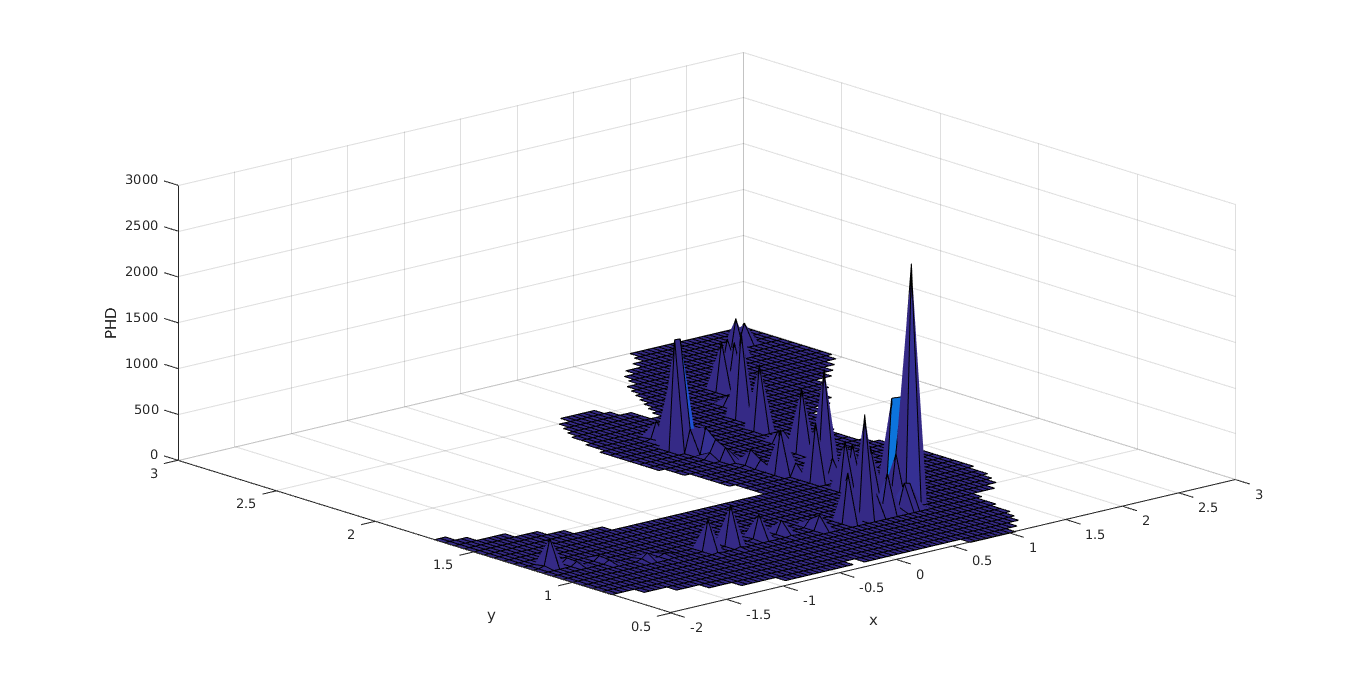
\includegraphics[width=0.8\linewidth]{include/images/phd_example.png}
\caption{example PHD visualization following three targets in the x-y state space over 20 time steps}
\label{fig:phd_example}
\end{figure}

The PHD filter propagates the PHD of the state RFS $X_k$ over time. $X_k$ is thus a random set containing the tracked targets at time step $k$. When both the motion and measurement model are linear and all noise on the models is gaussian then those elements are simply gaussian components described by their mean and covariance. The spikes seen in Figure \ref{fig:phd_example} are the gaussian components present throughout all time steps in the simulation. For every time-step $k$ the PHD therefore describes the intensity of this multimodal distribution and is denoted as $\upsilon_k(x)$.

There are several assumptions that have to be considered in order to be able to derive a recursive solution for propagating the PHD $\upsilon_k(x)$:

\begin{itemize}
    \item the targets move independently of each other
    \item clutter is poisson-distributed and independent of real observations
    \item the predicted RFS described by $p_{k|k-1}$ is poisson-distributed
\end{itemize}

Assuming that the predicted RFS is poisson-distributed is important because a poisson distribution is completely described by it's intensity. In a poisson distribution, the first moment (the mean) is denoted as $\lambda$ and all other moments can be derived from it.\todo{reference?} The prediction and update step for recursively computing the PHD are then as follows.\cite{Vo2006PHD}

\begin{equation}
    \begin{split}
        \upsilon_{k|k-1}(x) &= \int p_{S,k}(x_{k-1})f_{k|k-1}(x_k|x_{k-1})v_{k-1}(x_{k-1})dx_{k-1} \\
        &+ \int \beta_{k|k-1})(x_k|x_{k-1})v_{k-1}(x_{k-1})dx_{k-1} + \gamma_k(x) \\
        \upsilon_{k}(x) &= [1-p_{D,k}(x)]\upsilon_{k|k-1}(x) \\
        &+ \sum\limits_{z \in Z_k} \frac{p_{D,k}(x)g_k(z|x)\upsilon_{k|k-1}(x)}{\kappa_k(z) + \int p_{D,k}(x_{k|k-1})g_k(z|x_{k|k-1})\upsilon_{k|k-1}(x_{k|k-1})dx_{k|k-1}}
    \end{split}
\end{equation}

This recursion doesn't allow for a closed-form solution in the general case. However, a solution exists for the more specific case of linear motion and measurement models and considering only gaussian noise on the models.

\subsubsection{PHD Filter For The Linear And Gaussian Case}

Assuming linear models and only gaussian noise, the following state transition $f_{k|k-1}(x_k|x_{k-1})$ and likelihood $g_k(z|x_k)$ can be formulated. The variables are analogous to the ones used in the general motion and measurement model for the single-target tracking case described in equation \eqref{eq:motion_meas}.

\begin{equation}
    \begin{split}
        f_{k|k-1}(x_k|x_{k-1}) &= \mathcal{N}(x_k; F_{k-1}m_{k-1}, Q_{k-1} + F_{k-1}P_{k-1}F_{k-1}^T) \\
        g_{k}(z_k|x_{k}) &= \mathcal{N}(z_k; H_{k}m_{k|k-1},R_{k}+H_{k}P_{k|k-1}H_{k}^T)
    \end{split}
    \label{eq:gauss_phd_models}
\end{equation}

The resulting gaussian distribution is the central element in the linear, gaussian formulation of the PHD filter. Both the state RFS $X_k$ and the measurement RFS $Z_k$ consist of those gaussian components. This multimodal distribution over the state space for every time-step $k$ is what can be seen in Figure \ref{fig:phd_example}.

Since the Bayesian recursion always needs prior information to work on, a birth RFS $\gamma_k(x)$ has to be defined. The components in the birth RFS describe "areas" \todo{word choice? How about "regions"?} on the state-space in which new targets are most likely to appear. This could e.g. be an airport in the case of a flight-surveillance system or the borders of the sensor-range around an autonomous car that wants to track new objects coming into view. The birth RFS is a multimodal distribution comprised of a number of gaussian components.\cite{Vo2006PHD}

\begin{equation}
    \gamma_k(x) = \sum\limits_{i=1}^{J_{\gamma,k}} w^{(i)}_{\gamma,k} \mathcal{N}(x_k; m^{(i)}_{\gamma,k}, P^{(i)}_{\gamma,k})
\end{equation}

The mean and covariance of the gaussian components are used to position the distribution in the state-space and the weight $w^{(i)}_{\gamma,k}$ is used to determine the expected number of targets within that distribution. $J_{\gamma,k}$ is simply the number of components in the set. Just like the gaussian components, their associated weights will subsequently be updated in the Bayesian recursion and are then used to identify the most likely target states. 

Now, assuming that the posterior PHD at time $k-1$ was a multimodal gaussian distribution

\begin{equation}
    \upsilon_{k-1}(x) = \sum\limits_{i=1}^{J_{k-1}} w^{(i)}_{k-1} \mathcal{N}(x_k; m^{(i)}_{k-1},P^{(i)}_{k-1})    
\end{equation}

the predicted PHD at time $k$ is a multimodal gaussian distribution as well

\begin{equation}
    \upsilon_{k|k-1}(x) = \upsilon_{S,k|k-1}(x) + \gamma_k(x)    
\end{equation}

i.e. the predictions of the surviving targets from $k-1$ and the new births at $k$. Previous targets survive according to the defined survival probability $p_{S,k}$ and their next state is predicted according to the motion model defined in equation \eqref{eq:gauss_phd_models}.

\begin{equation}
    \upsilon_{S,k|k-1}(x) = \sum\limits_{j=1}^{J_{k-1}} w^{(j)}_{k-1} \mathcal{N}(x_k; m^{(j)}_{S,k|k-1},P^{(j)}_{S,k|k-1})   
\end{equation}

From this multimodal gaussian prediction, the update to the posterior can now be calculated as a sum of two terms. The first consists of all predictions assuming they were not detected as measurements at step $k$ and therefore downweighted. The second term assumes that all predictions actually are detected and updates them towards each of the measurements received at step $k$ analogous to a Kalman update.\cite{clark2006gm}

\begin{equation}
    \begin{split}
        \upsilon_k(x) &= (1-p_{D,k}) \upsilon_{k|k-1}(x) + \sum\limits_{z \in Z_k} \upsilon_{D,k}(x_k;z_k) \\
        \upsilon_{D,k}(x_k;z_k) &= \sum\limits_{j=1}^{J_{k|k-1}}w_k^{(j)}(z) \mathcal{N}(x_k; m^{(j)}_{k|k}(z_k),P^{(j)}_{k|k})\\
        w_k^{(j)}(z_k) &= \frac{p_{D,k}w^{(j)}_{k|k-1}q_k^{(j)}(z_k)} {\kappa_k(z_k)+p_{D,k}\sum\limits_{l=1}^{J_{k|k-1}}w^{(l)}_{k|k-1}q_k^{(l)}(z_k)}\\
        q_k^{(j)}(z_k) &= \mathcal{N}(z_k; H_{k}m_{k|k-1},R_{k}+H_{k}P_{k|k-1}H_{k}^T)\\
        m^{(j)}_{k|k}(z_k) &= m^{(j)}_{k|k-1} + K_k^{(j)}(z_k - H_k m^{(j)}_{k|k-1})\\
        P^{(j)}_{k|k} &= [I - K_k^{(j)}H_k]P^{(j)}_{k|k-1}\\
        K_k^{(j)} &= P^{(j)}_{k|k-1}H_k^T (H_k P^{(j)}_{k|k-1} H_k^T + R_k)^{-1}
    \end{split}
\end{equation}

As mentioned before, apart from propagating the PHD of the state RFS, the PHD filter is also used to recursively update the weight associated with each gaussian component. Those can then be used to estimate the number of targets present in the current time-step $\hat{N}_k$. Given a previous estimate $\hat{N}_{k|k-1}$ (or an initial estimate for $k=0$) the current estimate can be computed in the following way.\cite{Vo2006PHD}

\begin{equation}
\begin{split}
    \hat{N}_{k|k-1} &= p_{S,k}\hat{N}_{k-1} + \sum\limits_{j=1}^{J_{\gamma,k}} w^{(j)}_{\gamma,k}\\
    \hat{N}_k &= (1-p_{D,k})\hat{N}_{k|k-1} + \sum\limits_{z_k \in Z_k} \sum\limits_{j=1}^{J_{k|k-1}} w_k^{(j)}(z_k)
\end{split}
\end{equation}

Thus the PHD filter can be used to jointly estimate the number of targets and their states.

\todo{write about implementation issues in implementation part, e.g. assuming a poisson distributed RFS posterior, pruning, merging, tracking}

\newpage
\section{Extended Target Tracking}
The different Bayesian state estimation methods presented in sections \ref{sec:STT}-\ref{sec:RFS} are all introduced based on the assumption of dealing with point targets - targets that generate at most one measurement per sensor scan. In practice however, especially when using a range sensor such as a lidar, multiple measurements may arise from a target, especially when targets are relatively near the sensor. Such targets are commonly referred to as \emph{Extended Targets}. The distribution of lidar distance measurements arising from a target is dependent on which section of the targets spatial extent is within sensor view. As such, at any given sensor scan only a subset of the extended target will be seen. 

A simplistic approach when dealing with multiple measurements arising from a target is to calculate the mean value of all measurement. This enables the extended target to be treated as a point target. Such a method is suitable when dealing with targets whose spatial extent is relatively small, or in cases where the entire extended target is seen in the sensor field of view. However, large and partially viewed extended targets require more complex methods. Calculating the mean value of measurements will result in a loss of information about the spatial extent, as well as induce large estimation errors for a target's state. An illustrative example can be seen in Figure \ref{fig:spatialExample}. 

\begin{figure}[ht]
    \centering
    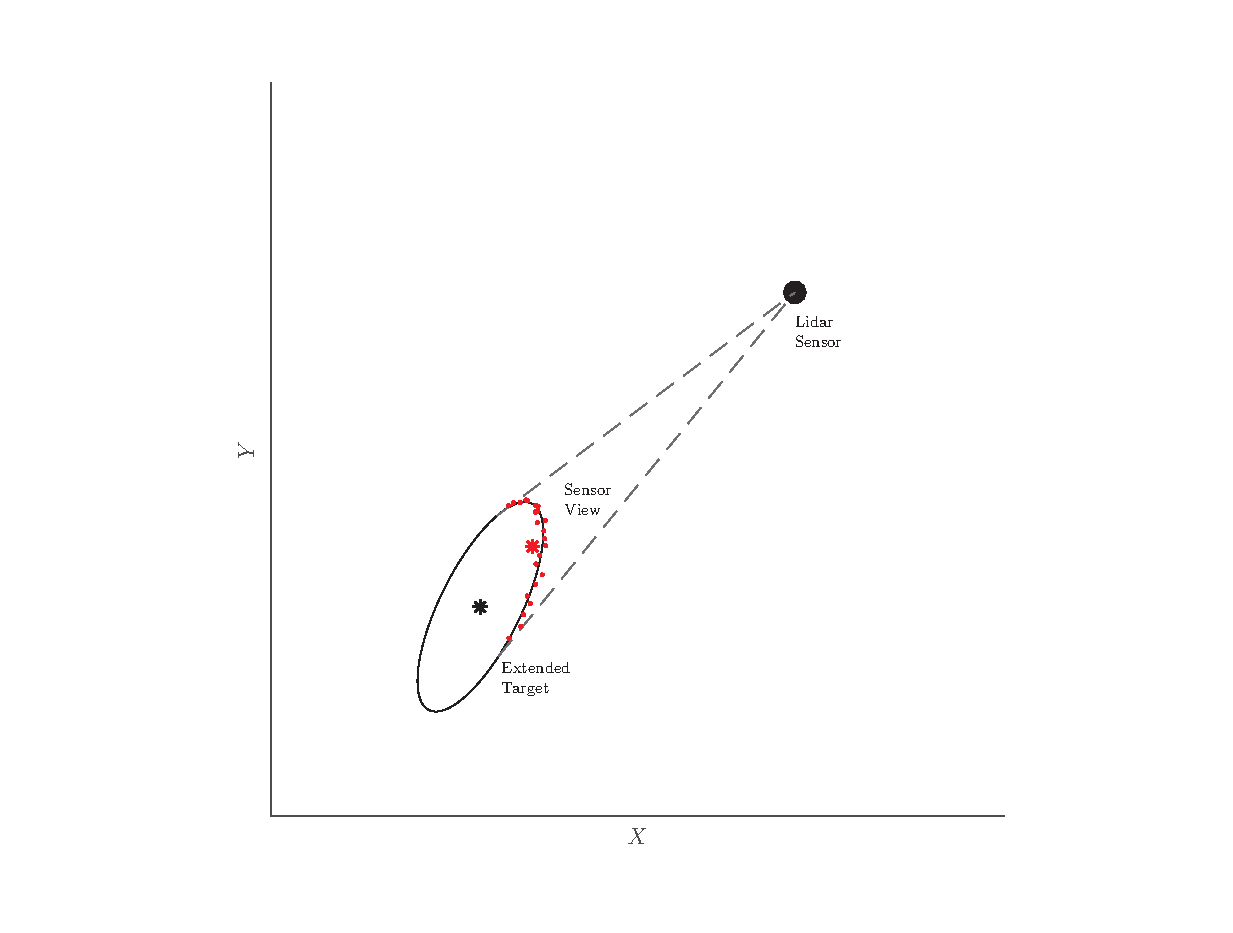
\includegraphics[width = 0.8\linewidth]{include/images/spatialExample.eps}
    \caption{An example of how an extended target with elliptical shape is viewed by a Lidar sensor. The red x's indicate measurements generated by the lidar Sensor. The small black circle denotes the center point of the Extended target, and the red small circle denotes the mean value of all measurements.}
    \label{fig:spatialExample}
\end{figure}

Here the extended target has an elliptical shape, but only a circular sector is seen from the sensor's field of view. Calculating the mean of all received measurements (the red exes) and treating it as a single measurement (the red circle) of the target's center point will yield a far more inaccurate measurement than the inherent inaccuracy for each individual measurement. Changes in for example heading for the elliptical target would be seen as changes in position, even though the target might not have necessarily performed any translative movement. Additionally, calculating target extent based solely on the spread of received measurements will underestimate the true spatial extent of the target. By not utilizing prior knowledge or intuition about shape, or past spatial distributions of measurements during a time sequence of a target, all severely limit the practical usefulness of the method.

In order to accurately estimate the behaviour of extended targets more robust techniques need to be considered, where a target's size and shape is considered. The following sections describe two different ways of dealing with extended targets: assuming rectangular shape and by utilizing random matrices.

\subsection{Tracking Under Assumed Rectangle Shape}

Rectangular shape modelling of targets is a suitable simplified model for describing the spatial extent of vehicles in cases where the shape of the car can be estimated to a high degree. By incorporating two additional parameters into the state vector, rectangle length $l$ and width $w$, the extended state vector can be formulated as

\begin{equation}
    \begin{split}
        \xi &=  
            \begin{bmatrix}
            x \\ 
            w \\ 
            l
            \end{bmatrix}
    \end{split}
\end{equation}

In order to incorporate tracking of extended rectangular targets, an analytical expression of the likelihood must be formulated. For a set $Z = \{z^{(j)}\}_{j=1}^{|Z|}$ of measurements, the likelihood can be expressed as 

\begin{equation}
    \begin{split}
        p(Z|\xi) = p(z^{(1)},z^{(2)},\dots,z^{(|Z|)}|\xi)
    \end{split}
\end{equation}

By treating each measurement as random independent variable drawn from a shape-dependent distribution, the joint likelihood can instead be expressed as the product of each individual measurement likelihood

\begin{equation}
    \begin{split}
        p(Z|\xi) &= \prod\limits_{j=1}^{|Z|} p(z^{(j)}|\xi)
    \end{split}\label{eq:zprod}
\end{equation}

The shape-dependent distribution can be approximated with a Gaussian mixture (GM) model, where the weights of the mixture sum to unity. The number of components $N_c$ in the GM govern how well the mixture approximates the true underlying distribution, where $N_c \rightarrow \infty$ asymptotically approximates the distribution completely. For a rectangular shape, the GM approach results in placing $N_c$ Gaussian kernels along the sides of a rectangle.

\begin{align}
    p(z^{(j)}|\xi) &\approx \sum\limits_{i=1}^{N_c} w^{(i)}\mathcal{N}(z^{(j)};\mu^{(i)}(\xi),\Sigma^{(i)}(\xi)), &  \sum\limits_{i=1}^{N_c} w^{(i)} &= 1 \label{eq:mix}
\end{align}

The two equations \eqref{eq:zprod} and \eqref{eq:mix} give sufficient analytical expressions for handling extended targets in a Bayesian fashion. By collapsing the GM to just consisting of a single component, each measurement $z^{(j)}$ can be seen as arising from a measurement generating point (MGP). As such, $\mu^{(i)}(\xi)$ represents a non-linear function describing the location of the MGP as dependent on the state $\xi$.

A benefit with this approach is that it allows \eqref{eq:zprod} to be expressed in the form of \eqref{eq:zconcat}, where $z_{Z}, \mu_{Z}(\xi)$ are vertical concatenations of all measurements and associated MGPs in the set $Z$, and $n_z$ is the number of measurements arising from each MGP. This enables the use of standard KF equations for prediction and estimation, negating the use of sequential Monte Carlo (particle filter) methods to evaluate the general forms expressed in \eqref{eq:zprod} and \eqref{eq:mix}. 

\begin{equation}
    \begin{split}
        p(Z|\xi) &= \prod\limits_{j=1}^{|Z|} \mathcal{N}(z^{(j)};\mu(\xi),\Sigma(\xi)) = \mathcal{N}(z_{Z}; \mu_{Z}(\xi), \sigma^2_{\Sigma}I_{n_z|Z|}) \\
            z_{Z} &= [z^{(1)}, z^{(2)}, \hdots, z^{(|Z|)}]^T \\
        \mu_{Z}(\xi) &= [\mu(\xi)^{(1)}, \mu(\xi)^{(2)}, \hdots, \mu(\xi)^{(|Z|)}]^T
    \end{split}\label{eq:zconcat}
\end{equation}

However, a difficulty with \eqref{eq:zconcat} is that it introduces an association problem, since each measurement $z^{(i)}$ must be associated to a corresponding MGP $\mu(\xi)^{(i)}$. A solution to the association problem can be found in REF, however such a solution requires measurements to be sorted according to bearing and incorporates all measurements, making such a method computationally intensive for a high number of measurements\todo{include reference to Karls article}. The solution to the association problem in this thesis is presented in section XXX \todo{refer to implementation section, where the practicalities of rectangular tracking are specified}.

The state of a rectangular target can be (minimally) described as consisting of positional coordinates $x$ and $y$, for example specifying the center point of the target. This makes it possible to express the positional coordinates in terms of the rectangle length $l$ and width $w$, which are also included in the state vector. Additionally, rotation of the rectangle can be described by its heading $\phi$.

\begin{equation}
    \begin{split}
        \xi_{\text{\tiny{min}}} &= [x\enskip y\enskip  \phi\enskip  w\enskip  l]^T
    \end{split}
\end{equation}

\begin{figure}[H]
    \centering
    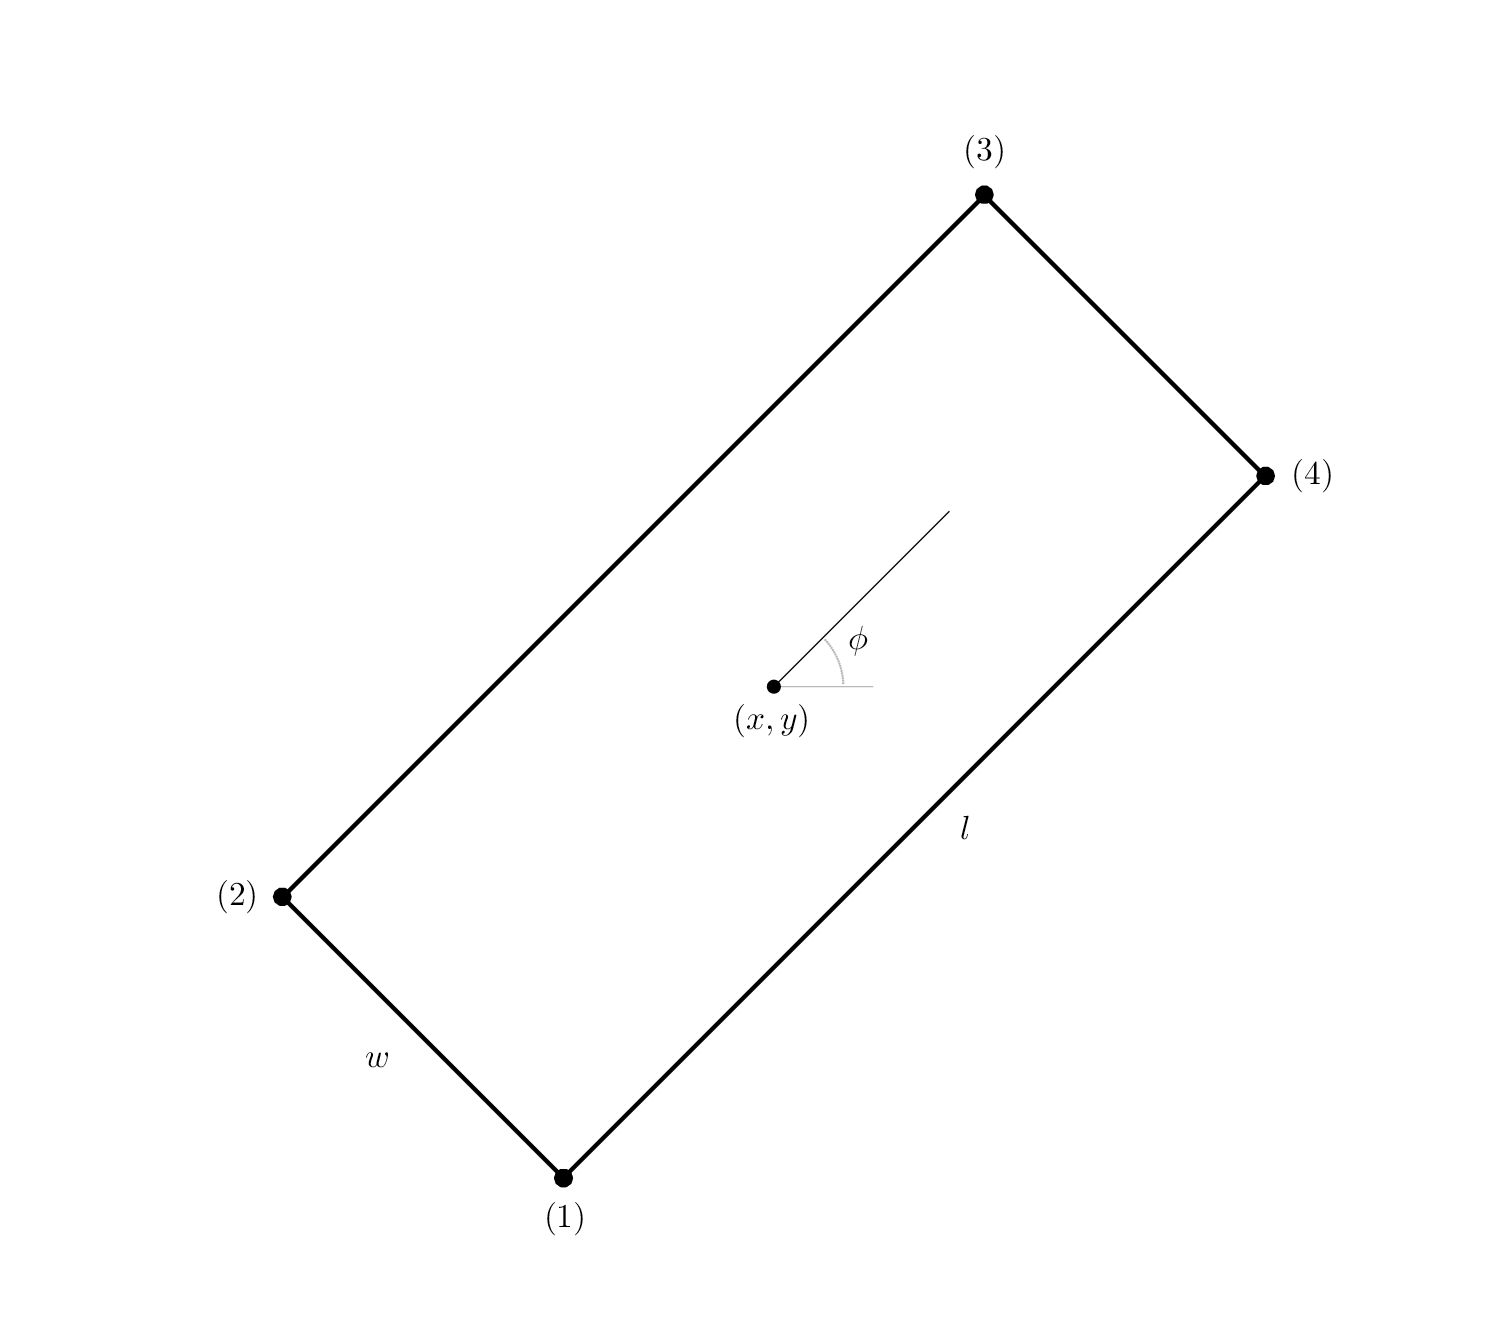
\includegraphics[width = 0.6\linewidth]{include/images/recFin.png}
    \caption{Car modelled as a rectangular shape.}
    \label{fig:spatialExample}
\end{figure}

Since each MGP is a function dependent on state, $\mu(\xi)$, any arbitrary point along any of the sides of the rectangle must be expressed in terms of the components in the state vector. For any scan, either one or two sides of a car will be seen by the range sensor. As such, each corner position $\{h_{c}^{i}\}_{i=1}^4$ of the rectangle, visualized in Figure \ref{fig:spatialExample}, can be used as a the base component for describing any arbitrary point along any of the rectangle's sides. For a rectangle where $x$ and $y$ are defined as being placed in the center of the rectangular shape, each corner position can be expressed as 

\begin{equation}
    \begin{split}
        h^{1}_{c}(\xi_{\text{\tiny{min}}})
            &= 
        \begin{bmatrix}
            x-\frac{1}{2}\sqrt{(w^2 + l^2)} \cos(\arctan(w/l) + \phi) \\
            y-\frac{1}{2}\sqrt{(w^2 + l^2)} \sin(\arctan(w/l) + \phi)
        \end{bmatrix} 
        \\
        h^{2}_{c}(\xi_{\text{\tiny{min}}})
            &= 
        h^{1}_{c}(\xi_{\text{\tiny{min}}})
        + 
        \begin{bmatrix}
            w \cos(\phi +\pi/4) \\
            w \sin(\phi +\pi/4)
        \end{bmatrix}
        \\
        h^{3}_{c}(\xi_{\text{\tiny{min}}})
            &= 
        h^{2}_{c}(\xi_{\text{\tiny{min}}})
        + 
        \begin{bmatrix}
            l \cos(\phi) \\
            l \sin(\phi)
        \end{bmatrix}
        \\
        h^{4}_{c}(\xi_{\text{\tiny{min}}})
            &= 
        h^{1}_{c}(\xi_{\text{\tiny{min}}})
        + 
        \begin{bmatrix}
            l \cos(\phi) \\
            l \sin(\phi)
        \end{bmatrix}
    \end{split}
\end{equation}

Considering how range sensors work, a reasonable assumption is that measurements are uniformly distributed along each visible side of the rectangle. As such the position for $N_{\text{\tiny{MGP}}}$ uniformly distributed MGPs along the width or length, relative to corner $i$, can be described by

\begin{align}
    \{h_{l}^j(\xi_{\text{\tiny{min}}})\}_{j = 1}^{N_{\text{\tiny{MGP}}}} &= h_c^i(\xi_{\text{\tiny{min}}}) + \frac{j}{1+N_{\text{\tiny{MGP}}}}\rho_l
        \begin{bmatrix}
            l\cos(\phi + \eta(i)) \\
            l\sin(\phi + \eta(i)) 
        \end{bmatrix}, & \eta(i) &\rightarrow \{0,0,\pi,\pi\} 
    \\\nonumber 
    \\ 
    \{h_{w}^j(\xi_{\text{\tiny{min}}})\}_{j = 1}^{N_{\text{\tiny{MGP}}}} &= h_c^i(\xi_{\text{\tiny{min}}}) + \frac{j}{1+N_{\text{\tiny{MGP}}}}\rho_w
    \begin{bmatrix}
        w\cos(\phi + \eta(i)) \\
        w\sin(\phi + \eta(i)) 
    \end{bmatrix}, & \eta(i) &\rightarrow \left\{\frac{\pi}{2},\frac{3\pi}{2},\frac{3\pi}{2},\frac{\pi}{2}\right\} 
\end{align}

Where $0\leq\rho_w,\rho_l\leq1$ represents how much of each side is in view of the sensor. This is an important parameter, since in practice range sensor may not see the entire side due to factors such as reflectivity or range to target. As such, distributing MGPs only along the viewed length and width is necessary in order to get good estimates of shape and (by extension) kinematic state.

\subsection{Tracking With Random Matrices}

The rectangular shape model for cars is very specifically tailored for that particular use case. This, however, makes it impractical to use with other objects that don't show such a shape or general behaviour that can be accurately described by the state vector introduced in \todo{link to Marko's x,y,dx,dy,phi,w,l state vector}. Since this thesis is not only concerned with tracking cars but also other common traffic participants (namely pedestrians and cyclists), an efficient model for estimating their form had to be found.

It is worth pointing out a principal difference of how cars and both pedestrians and cyclists usually show their extent in lidar data. In general a car is a solid object that is much longer and wider than a pedestrians or cyclist. It therefore has the potential to block out quite a lot of it's shape from the sensor view itself. It does not have to be blocked from view by some other object, it actually hides parts of itself. An example of that can be observed in Figure \ref{fig:car_extended_target}.

\begin{figure}[H]
\centering
\begin{subfigure}{.5\textwidth}
  \centering
  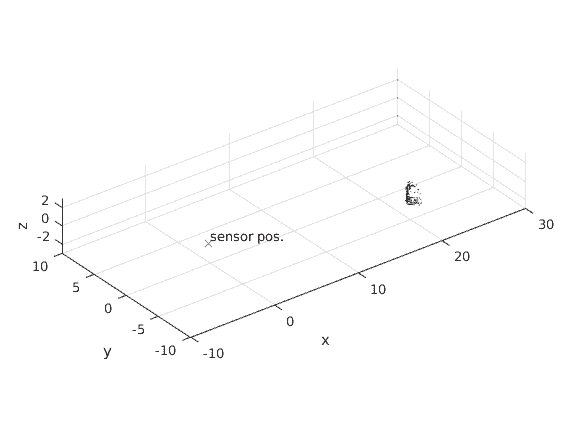
\includegraphics[width=1.0\linewidth]{include/images/car_extended_target_ex1.png}
\end{subfigure}%
\begin{subfigure}{.5\textwidth}
  \centering
  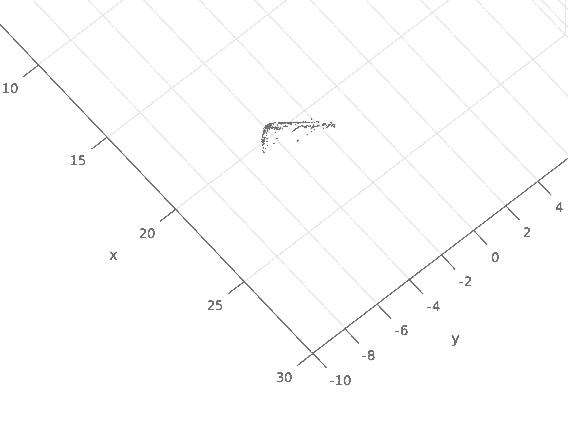
\includegraphics[width=1.0\linewidth]{include/images/car_extended_target_ex2.png}
\end{subfigure}
\caption{a car blocking parts of it's own extent from the sensor view, isometric and top-down perspective}
\label{fig:car_extended_target}
\end{figure}

Since a car has relatively large dimensions, this leads to actually loosing a lot of information about the target which is why the proposed rectangular tracking method is so important to get a better estimate of a car's true center position. Fortunately this doesn't hold true for cyclists and pedestrians. They are much smaller in size and thus their extent shows up pretty much directly in the lidar data. This can be seen for the case of a cyclist in Figure \ref{fig:cycle_extended_target}. As pedestrians are smaller still, this holds true even more for them.

\begin{figure}[H]
\centering
\begin{subfigure}{.5\textwidth}
  \centering
  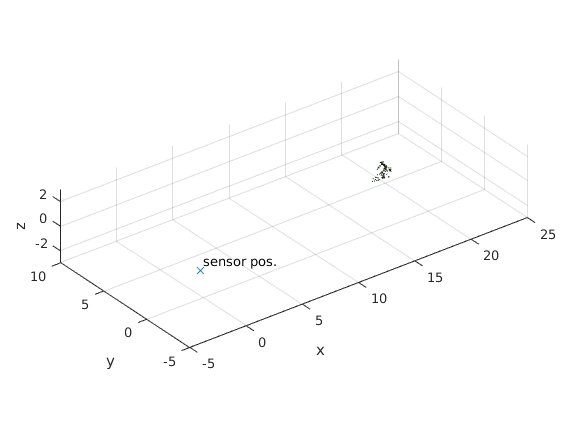
\includegraphics[width=1.0\linewidth]{include/images/cycle_extended_target_ex1.png}
\end{subfigure}%
\begin{subfigure}{.5\textwidth}
  \centering
  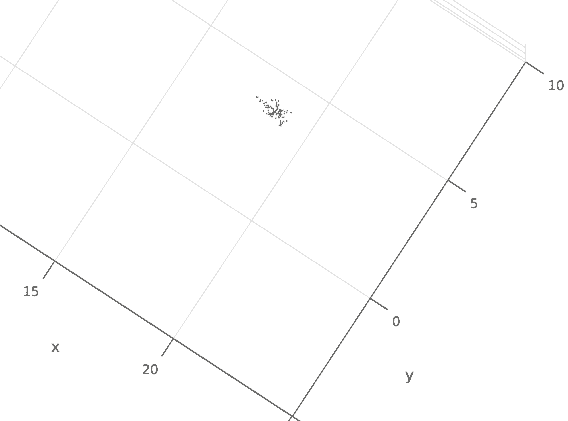
\includegraphics[width=1.0\linewidth]{include/images/cycle_extended_target_ex2.png}
\end{subfigure}
\caption{a cyclist showing it's true extent very clearly directly in the lidar data, isometric and top-down perspective}
\label{fig:cycle_extended_target}
\end{figure}

It is therefore a reasonable approach to simply track the extent of a pedestrian or cyclist that shows up in the data in order to get a sufficiently good estimate of their true form. As is turns out, the shape of both of those targets can be approximated accurately by ellipses. While being very versatile and able to cover many different forms by adjusting length, width and eccentricity, ellipses are easy to model and incorporate into a tracking framework. Koch who first used elliptical target tracking within a Bayesian formalism describes that ellipses can effectively be used to track the size, shape and orientation of an extended target. \cite{koch2008elliptical}

Koch introduces an extended state vector 

\begin{equation}
    \xi = [\vec{x}_k^T, \vec{X}_k^T]^T
\end{equation}

that models both the kinematic state $\vec{x}_k$ of a target (e.g. position, velocity, acceleration) as well as the target extent $\vec{X}_k$ which contains the parameters needed to define the ellipse. $\vec{X}_k$ in the Bayesian framework is a random variable and can be modelled as a random matrix drawn from an inverse Wishart distribution. \cite{koch2008elliptical}

Considering the elliptical shape of the level curves of the covariance matrix in a 2-dimensional Gaussian distribution it becomes clear how an ellipse shape can be derived from a random positive-definite matrix. This is also why it can be modelled as an inverse Wishart distribution: it is a probability distribution over positive-definite matrices. It can be used as a conjugate prior to estimate the random matrix that defines the extent ellipse. \cite{barberBRML2014} Using it as a conjugate prior ensures that the random matrix will, throughout the entire filter recursion, remain inverse Wishart distributed. Drawing a sample from it will therefore always result in obtaining a positive-definite matrix. \todo{do we need to go deeper here and explain why it needs to be positive-definite in order to derive the elliptical level curves?}

An inverse Wishart distribution is described by the following probability density function

\begin{equation}
    p(X|v,V) = \frac{|V|^\frac{v}{2}}{2^\frac{vd}{2}\Gamma_d(\frac{v}{2})}|X|^{-\frac{v+d-1}{2}}e^{-\frac{1}{2}tr(VX^{-1})}
\end{equation}

where $\Gamma_d$ is the multivariate gamma function, $tr$ is the trace function, $d$ is the size $d \times d$ of $X$, $v$ is the degrees of freedom of the distribution and $V$ is the positive definite scale matrix. The expected value of a draw from this distribution is defined as

\begin{equation}
    E[X] = \frac{V}{v-d-1}
    \label{eq:exp_iwish}
\end{equation}

As you can see, the probability density function is parametrized by $v$ and $V$. To get a more intuitive understanding of what kind of ellipses to expect from a draw from an inverse Wishart distribution it is useful to visualize some samples for varying degrees of freedom $v$. Equation \eqref{eq:exp_iwish} states that the expected value is the scale matrix $V$ scaled down by the degrees of freedom $v$ subtracted with the dimensions $d$ and 1. The expected value for a sample drawn from an inverse Wishart distribution therefore diminishes for an increasing $v$. This can be seen in Figure \ref{fig:iwish_parameters_ex}. On top of that the variance in the samples decreases, such that they converge simply to a scaled down version of $V$ with little variation in orientation or eccentricity.

\begin{figure}[H]
    \centering
    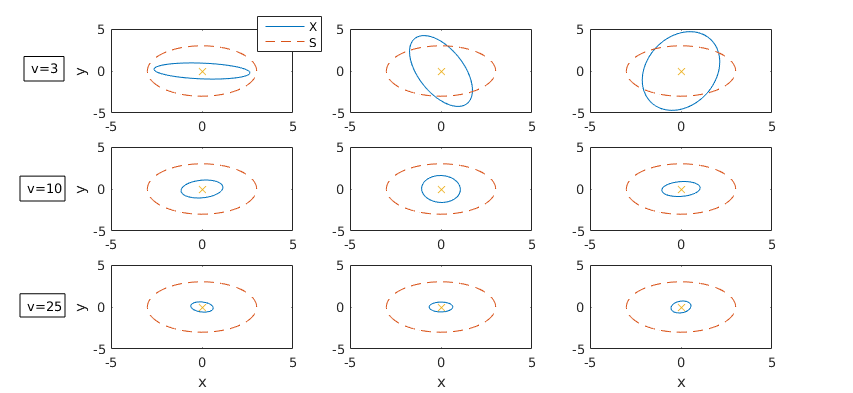
\includegraphics[width=0.9\linewidth]{include/images/iwish_parameters_ex.png}
    \caption{9 inverse Wishart distribution samples for varying degrees of freedom $v = \{3,10,25\}$ and constant $V = diag([1,1])$}
    \label{fig:iwish_parameters_ex}
\end{figure}

A closed-form Bayesian recursion to propagate both the kinematic state $\vec{x}_k$ and the extent of a target $\vec{X}_k$ was developed by Koch in \cite{koch2008elliptical}. It follows the usual Bayesian filtering steps of prediction through a motion model and update through a likelihood function based on a measurement model. The kinematic state is modeled as a Gaussian distribution parametrized by the mean $x_k$ and covariance $P_k$, while the extent is modelled as an inverse Wishart distribution as described before.

\textbf{Prediction} \\
The kinematic part:
\begin{equation}
\begin{split}
    x_{k|k-1} &= (F_{k|k-1} \otimes I_d)x_{k-1|k-1}\\
    P_{k|k-1} &= F_{k|k-1}P_{k|k-1}F_{k|k-1}^T + Q_{k|k-1}
\end{split}
\label{eq:ellip_prediction_kin}
\end{equation}

The extent part:
\begin{equation}
\begin{split}
    v_{k|k-1} &= e^{\frac{-T}{\tau}} v_{k-1|k-1}\\
    V_{k|k-1} &= \frac{e^{\frac{-T}{\tau}}v_{k-1|k-1}-d-1}{v_{k-1|k-1}-d-1}V_{k-1|k-1}
\end{split}
\label{eq:ellip_prediction_ext}
\end{equation}

Here $T$ is the step time of the process and $\tau$ a decay constant that is used to steer how much both $v$ and $V$ decrease in the prediction step. Lower values for $v$ and $V$ can be interpreted as a higher uncertainty in the estimations drawn from the distribution, as illustrated in Figure \ref{fig:iwish_parameters_ex}. $I_d$ is the identity matrix of dimension $d$.

\textbf{Update} \\
The center $z_k$ and scatter matrix $Z_k$ of a measurement cluster with $n_k$ measurements:
\begin{equation}
\begin{split}
    z_k &= \frac{1}{n_k}\sum\limits_{j=1}^{n_k} z_k^j \\
    Z_k &= \sum\limits_{j=1}^{n_k}(z_k^j - z_k)(z_k^j - z_k)^T
\end{split}
\label{eq:ellip_meas_init}
\end{equation}

The kinematic part:
\begin{equation}
\begin{split}
    S_{k|k-1} &= H_kP_{k|k-1}H_k^T + \frac{1}{n_k} \\
    K_{k|k-1} &= P_{k|k-1}H_k^TS_{k|k-1}^{-1} \\
    x_{k|k} &= x_{k|k-1} + (K_{k|k-1} \otimes I_d) (z_k - (H_k \otimes I_d) x_{k|k-1})\\
    P_{k|k} &= P_{k|k-1} - K_{k|k-1}S_{k|k-1}K_{k|k-1}^T
\end{split}
\label{eq:ellip_update_kin}
\end{equation}

Where $S_{k|k-1}$ is the innovation factor and $K_{k|k-1}$ is the gain.

The extent part:
\begin{equation}
\begin{split}
    N_{k|k-1} &= S_{k|k-1}^{-1} (z_k -(H_k \otimes I_d)x_{k|k-1}) z_k - (H_k \otimes I_d) x_{k|k-1})^T \\
    v_{k|k} &= v_{k|k-1} + n_k \\
    V_{k|k} &= V_{k|k-1} + N_{k|k-1} + Z_k
\end{split}
\label{eq:ellip_update_ext}
\end{equation}

Where $N_{k|k-1}$ is the innovation matrix.

For the derivation of these equations, details on the assumptions made and the theoretical background the reader is referred to \cite{koch2008elliptical}.

\subsubsection{Random Matrix PHD Filter}
The propagation of random matrices to estimate the extent of a target can be included into a basic PHD Filter framework as described in section 2.2.1 and 2.2.2 .\todo{dynamic linking} Instead of propagating a Gaussian mixture RFS there is now a Gaussian component (for the kinematic state) and an inverse Wishart component (for the extent) associated with every target. Granström and Orguner showed an implementation in \cite{granstrEllipPHD2012}.

The main problem to solve is to derive a suitable likelihood function that can be used to update the components' weights. Basically, based on the predictions about the kinematic state and the extent of a target and the measurements you receive you have to be able to decide which measurements fit which target best.

\textbf{Prediction}\\
At first, each of the $J_{k-1|k-1}$ existing prior component's weight is adjusted based on the survival probability $p_S$.

\begin{equation}
    w^{(i)}_{k|k-1} = P_sw^{(i)}_{k-1|k-1}, \forall i \in J_{k-1|k-1}
    \label{eq:giw_phd_weight_pred}
\end{equation}

\textbf{Update}\\
The update step is partitioned into two parts. In the case of no available measurement (no detection) for a particular target the weight is lowered:

\begin{equation}
    w^{(j)}_{k|k} = (1-(1-e^{-\gamma(j)})p_D^{(j)})w^{(j)}_{k|k-1}, \forall j \in J_{k|k-1}
    \label{eq:giw_phd_weight_update1}
\end{equation}

with $\gamma(j)$ being the expected number of measurements for that target.

Otherwise the weight is updated according to a likelihood function that says how well the shape and position of the predicted ellipse matches the position and shape of the updated ellipse. Every measurement $z_i \in Z_k$ is used to update and calculate a likelihood for every existing predicted target $j \in J_{k|k-1}$.

\begin{equation}
    w_{k|k}^{(j+J_{k|k-1}(i-1))} = \frac{e^{-\gamma^(j)}(\gamma^{(j)})^{|z_i|}p_D^{(j)}}{\beta_k^{|z_i|}(\pi^{|z_i|}|z_i|S)^{\frac{d}{2}}} \frac{|v_{k|k-1}^{(j)}|^{|v_{k|k-1}^{(j)}/2}}{|V_{k|k}^{(j+J_{k|k-1}(i-1))}|^{|V_{k|k}^{(j+J_{k|k-1}(i-1))}/2}} \frac{\Gamma_d(v_{k|k}^{(j+J_{k|k-1}(i-1))}/2)}{\Gamma_d(v_{k|k}^{j}/2)} w_{k|k-1}^{j}, \forall j \in J_{k|k-1}, \forall z_i \in Z_k
    \label{eq:giw_phd_weight_update2}
\end{equation}

with $\Gamma_d$ being the multivariate gamma function, $|z_i|$ being the number of points in measurement $z_i$ and $\beta_k$ being the expected number of clutter measurements in $Z_k$. Both $v_{k|k}^{(j+J_{k|k-1}(i-1))}$ and $V_{k|k}^{(j+J_{k|k-1}(i-1))}$ are the updated parameters of the inverse Wishart distribution, the computation of which can be seen in \cite{granstrEllipPHD2012}.

All updated predictions towards a certain measurement $z_i$ are normalized amongst themselves in the following way.

\begin{equation}
\begin{split}
    d_{z_i} &= \delta_{|z_i|,1} + \sum\limits_{j=1}^{J_{k|k-1}} w_{k|k}^{(j+J_{k|k-1}(i-1))}\\
    w_{k|k}^{(j+J_{k|k-1}(i-1))} &= \frac{w_{k|k}^{(j+J_{k|k-1}(i-1))}}{d_{z_i}}, \forall j \in J_{k|k-1}
    \label{eq:giw_phd_weight_norm}
\end{split}
\end{equation}

$\delta_{|z_i|,1}$ is the Kronecker delta which evaluates to $1$ if the two subscripts are equal or to $0$ otherwise.

For more details on this Gaussian inverse Wishart PHD (GIW-PHD) filter the reader is referred to the excellent article \cite{granstrEllipPHD2012} and the accompanying technical report \cite{giwphdtechnical} that provides pseudo-code for an implementation and also talks about implementation issues and the computational complexity of the filter.

\section{Neural Networks for Classification}
This section aims to explain the basic algorithms used by two common Machine Learning tools to solve classification tasks: Logistic Regression and Neural Networks. A Neural Network for classification can be seen as a combination of several logistic regression blocks. This explains the order in which the concepts are introduced. 

\subsection{Logistic Regression}
At the root of logistic regression lies the desire to find an appropriate function that defines a boundary between the different classes present in the data. In this thesis this is e.g. the decision whether a certain object is a car or not. An example of such a boundary can be seen on the left side in Figure \ref{fig:log_reg_ex} for a case where a linear function works well to separate the two areas. The green circles are examples for one class in the dataset, the blue crosses signify the other class. More difficult cases like the one shown on the right side in Figure \ref{fig:log_reg_ex} can't be separated by a linear function, a nonlinear function is needed to differentiate between them. For a growing complexity of separation between the different classes or a growing number of input dimensions (both examples are obviously just in 2D) more and more complex nonlinear functions have to be created in the network. \todo{can one nonlinear function be more nonlinear than another?}

\begin{figure}[H]
\centering
\begin{subfigure}{.5\textwidth}
  \centering
  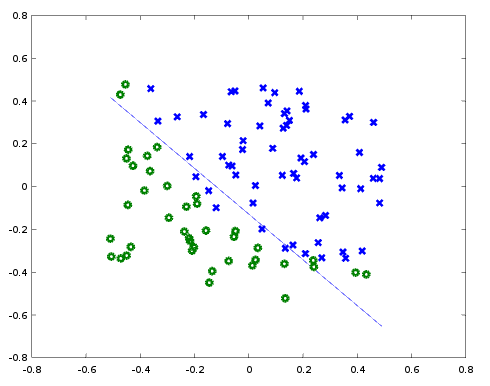
\includegraphics[width=1.0\linewidth]{include/images/logistic_regression_linear_ex.png}
  \label{fig:log_reg_lin_ex}
\end{subfigure}%
\begin{subfigure}{.5\textwidth}
  \centering
  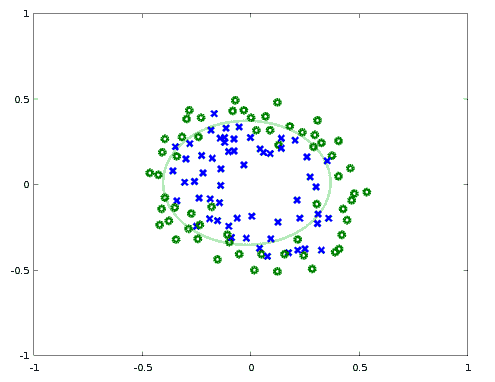
\includegraphics[width=1.0\linewidth]{include/images/logistic_regression_polynomial_ex.png}
  \label{fig:log_reg_pol_ex}
\end{subfigure}
\caption{logistic regression with a linear and a polynomial boundary}
\label{fig:log_reg_ex}
\end{figure}
\todo{use a better figure here: labels, add a nonlinear case also}

The x- and y-axes in Figure \ref{fig:log_reg_ex} are the so-called features of that particular classification problem. Features are carefully chosen properties of the objects to be classified. In this thesis this could e.g. be the density and the number of points in a point cluster. Obviously those features need to have somewhat unique values for the different classes in the dataset such that the respective examples (i.e. the datapoints in Figure \ref{fig:log_reg_ex}) actually end up in different parts of the plot and are therefore separable.

Plotting such datasets and their decision boundary is really only useful for the 2-dimensional (data with 2 features, separated by a line or curve) and 3-dimensional case (data with 3 features, separated by a plane or a curved plane). Humans generally lack the visualization for e.g. 4-dimensional features separated by a 3-dimensional plane. However, the following concepts and equations hold true for the general case of an n-dimensional space separated in the dimension of it's hyperspace.

\subsubsection{Logistic Regression Cost Function}

The optimal decision boundary between the different classes is found by optimizing a cost function which is a function of $\Theta$ and sums up the difference between the predicted outputs with that particular weight configuration $\Theta$ and the true outputs from the training data. A plot of an example cost function over two $\Theta$ values can be seen in Figure \ref{fig:surf_cost_function}. 

\begin{figure}[H]
\centering
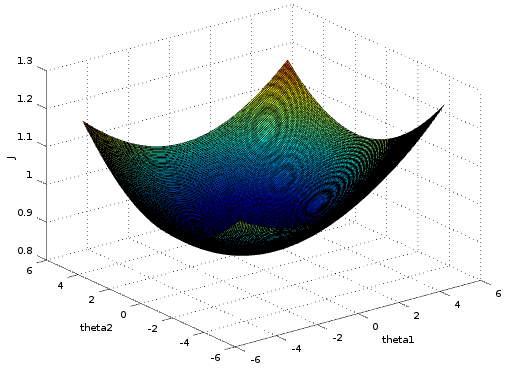
\includegraphics[width=0.8\linewidth]{include/images/surf_cost_function.png}
\caption{an example cost function $J(\Theta)$ over two values of $\Theta$}
\label{fig:surf_cost_function}
\end{figure}

The cost function in the case of logistic regression is as follows.

\begin{equation}
    J(\Theta) = \frac{1}{m} \left[\sum_{i=1}^m -y^{i} \log(h_\Theta(x^{(i)})) - 
    (1-y^{(i)} \log(1-h_\theta(x^{(i)}))\right]
    \label{eq:log_cost}
\end{equation}
\todo{somehow cite those equations to the coursera course or find a book where they are described in that way}

This equation includes the two distinct cases for being part of a certain class ($y=1$) and the other for not being part of that class ($y=0$).

\begin{equation}
J(\theta)= \frac{1}{m} \sum_{i=1}^m \begin{cases}
    y = 1, & -\log(h_\Theta(x))\\
    y = 0, & -\log(1-h_\Theta(x))
  \end{cases}
\end{equation}

If the true output $y$ is $1$ then the cost of the prediction $h_\Theta(x)$ is measured by the equation belonging to that case and the other way around if the true output $1$ is $0$. Considering the plots for both $-\log(x)$ and $-\log(1-x)$ in Figure \ref{fig:plot_neglog} it can be seen that the cost for predicting exactly the true output is zero but increases exponentially for deviations further and further away from the true output. 

\begin{figure}[H]
\centering
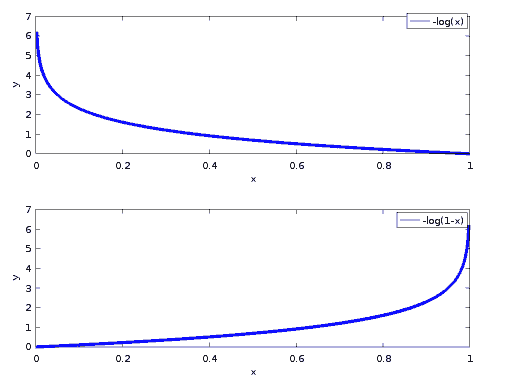
\includegraphics[width=0.8\linewidth]{include/images/plot_neglog.png}
\caption{both parts of the logistic regression cost function: $-\log(x)$ and $-\log(1-x)$}
\label{fig:plot_neglog}
\end{figure}
\todo{this plot is a bit ugly ;)}

The cost function $J(\Theta)$ simply sums up the cost for all examples a logistic regression classifier is being trained on. This is then the cost for a certain configuration of $\Theta$. The aim is now to try and find the values for $\Theta$ that render the lowest possible cost for $J(\Theta)$. Considering the plot of the cost function in Figure \ref{fig:surf_cost_function} you can see that you essentially want to find the bottom of that "bowl-shaped" function. 

As the logistic regression cost function in \eqref{eq:log_cost} is guaranteed to be convex \todo{do we need to prove that? or at least cite a source for that statement?} any minimum found is guaranteed to be the global minimum.

\subsubsection{Gradient Descent}

In order to find the minimum of the cost function $J(\Theta)$ a technique called gradient descent is used. An intuitive understanding of the algorithm can be gained by considering Figure \ref{fig:surf_cost_function} once more. The starting point would be a random configuration for $\Theta$. From there, you iteratively subtract the current gradient in all $\Theta$ directions. You will descend into the "bowl" until you reach the bottom. This can be expressed as follows.

\begin{equation}
\Theta_j = \Theta_j - \alpha \frac{\partial}{\partial \Theta_j} J(\Theta)
\end{equation}

Here $\Theta_j$ is the j-th element of the $\Theta$ vector and $\alpha$ is a learning parameter that controls the speed with which $J(\Theta)$ approaches it's minimum. Choosing $\alpha$ too low will result in a slow convergence towards the minimum while choosing $\alpha$ too high can result in missing the minimum and actually diverging. The partial derivate of of $J(\Theta)$ w.r.t a certain element of $\Theta$ is computed as:

\begin{equation}
\frac{\partial}{\partial \Theta_j} = \sum_{i=1}^m((h_\Theta(x^{(i)}) - y^{(i)})x_j^{(i)}
\end{equation}

Here $(i)$ denotes the $i$-th example in the dataset used to train the classifier which contains $m$ examples in total. $h_\Theta(x^{(i)})$ is therefore the $i$-th prediction based on the $i$-th feature-input and $y^{(i)}$ is the $i$-th true output to compare with. An example plot of this process of minimizing the cost over subsequent iterations of the gradient descent algorithm can be seen in Figure \ref{fig:plot_cost_function_over_iter}.

\begin{figure}[H]
\centering
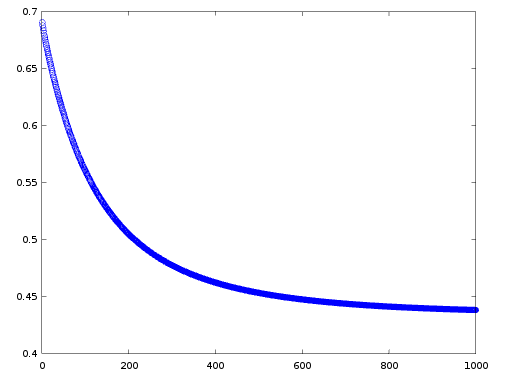
\includegraphics[width=0.8\linewidth]{include/images/plot_cost_function_over_iter.png}
\caption{example plot of a gradient descent algorithm}
\label{fig:plot_cost_function_over_iter}
\end{figure}
\todo{better plot, caption and labels}

\todo{add some differentiation between logistic regression and normal regression}

\subsection{Neural Network}
As a first approach a basic single hidden layer classification network was implemented for this thesis because it allows to adjust the complexity as needed (up to a certain degree) simply by adjusting the number of hidden units. It worked so well that a more complex structure was deemed not to be necessary. A single hidden layer neural network can be described in the following way.

A neural classification network is basically a nonlinear function mapping from an input matrix of features $X$ to an output vector of classifications $Y$. $X$ has $m$ rows and the number of columns corresponds to the number of features used. The length of $Y$ is $k$, with $k$ being the number of different classes to be classified.

\begin{equation}
    Y = f(X)
\end{equation}

The calculation of an output is done by processing the inputs through a neural network structure as depicted in Figure \ref{fig:nn_structure}. The structure of the network consists of 3 important building blocks: layers, units and connections. The layers are the horizontal groupings seen in the Figure. The first is the input layer, the second the hidden layer and the third the output layer. Every layer is made up of a number of units (the so-called neurons), drawn as the coloured circles in the Figure. Each neuron has several input connections from other neurons in the previous layer and one output connection to another neuron in the next layer. A connection always has a weight assigned to it. 

\begin{figure}[H]
\centering
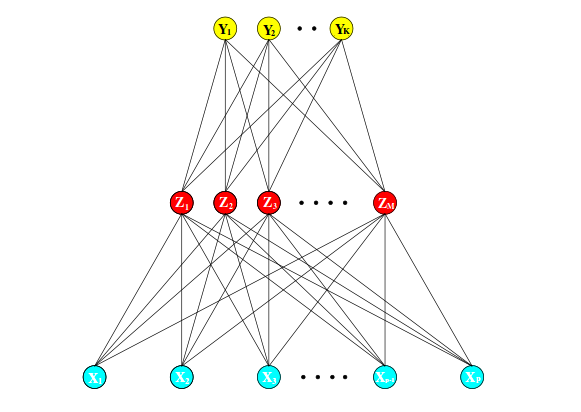
\includegraphics[width=0.8\linewidth]{include/images/nn_structure.png}
\caption{single hidden layer neural network structure\cite{hastie2009elements}}
\label{fig:nn_structure}
\end{figure}
\todo{use a better Figure that shows the weights as well}

The computation is done in two steps, each advancing one layer forward. As the input layer is given, the first step is to compute the values for the hidden layer. Each unit's value is determined as the linear combination of the respective input neurons' values times the weight of the connection. This value is then scaled to be between $0$ and $1$ by applying the sigmoid function to it. This function is called the activation function of the neuron.\todo{why is it scaled in that way? why not another function? it used to be a step function but that one is hard to optimize, sigmoid is smoother}

\begin{equation}
    \sigma = g(z) = \frac{1}{1+e^{-z}}
\end{equation}

A plot of the sigmoid function is shown in Figure \ref{fig:plot_sigmoid}.

\begin{figure}[H]
\centering
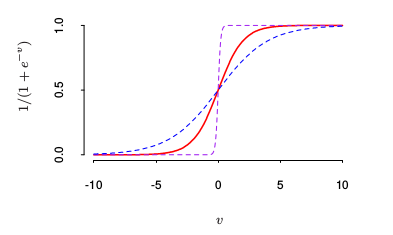
\includegraphics[width=0.8\linewidth]{include/images/plot_sigmoid.png}
\caption{sigmoid function with different scalings}
\label{fig:plot_sigmoid}
\end{figure}
\todo{use a better figure here: input is x, no scaling}

For example, the value of $Z_1$ would therefore be computed as

\begin{equation}
    Z_1 = \sigma(X_1\Theta_1^{11} + X_2\Theta_1^{21} + ... + X_P\Theta_1^{1P})
\end{equation}
\todo{is all the notation consistent between the figures and formulas}

with $\Theta_1$ being the weight matrix for each connection between the input layer and the hidden layer containing $p$ (number of input units) rows and $m$ (number of hidden units) columns.
\todo{insert figure with connections and weights between input and hidden and the corresponding weight matrix here}
\todo{adjust notation here to correspond to andrew ng's notation}

By writing all inputs as a matrix with each entry as one row vector $X = [X_1, X_2, ..., X_P]^T$ the entire computation can be vectorized and the vector of hidden units $Z$ be calculated in the following way. 

\begin{equation}
    Z = \sigma(\Theta_1^TX)
\end{equation}

The same procedure is repeated from the hidden layer $Z$ to the output layer 
$Y$ to reach the classification of the inputs.

\begin{equation}
    Y = \sigma(\Theta_2^TZ)
\end{equation}
\todo{this whole section should include a paragraph about the bias units as well}

As you can see from Figure \ref{fig:plot_sigmoid} the outputs will be values between $0$ and $1$ and describe the probability of the input to belong to that particular class signified by the respective unit in the output layer.

\todo{talk about supervised vs unsupervised learning}

\subsubsection{Training the Neural Network}

As can be seen from the equations and the principal structure of the network, there are basically 3 ways to influence the mapping from inputs $X_p$ to outputs $Y_k$:

\begin{itemize}
    \item number of hidden layers
    \item number of units in the hidden layers
    \item connection weights
\end{itemize}

As described earlier, in this thesis the decision was made to focus on a simple network structure with a single hidden layer and a fixed number of hidden units. Initial tests showed promising results even with those limitations and therefore there was no reason to dive into a more complex configuration.

\subsubsection{Backpropagation}

With a fixed number of layers and units in the network, the only way to change it's output is to adjust the weights of the connections $\Theta$. Similarly to the gradient descent algorithm described to calculate the optimal values for $\Theta$ in logistic regression, there is a process to derive the optimal $\Theta$ configuration for a neural network: backpropagation.

\todo{use correct layer notation here and show size of $\Theta$ matrices}
The intuition behind it is similar to gradient descent - the aim is to minimize a cost function. However, instead of one $\Theta$ vector mapping the inputs $X$ to the predictions $h_\Theta(X)$ there are now two $\Theta$ matrices each describing the weights from one layer to the next. Each of these $\Theta$ matrices is made up of several vectors each containing the weights of all units in layer $l$ to a particular unit in $l+1$. 

Optimizing the entire neural network's $\Theta$ configuration can therefore be seen as a combination of several local optimizations between the layers. Backpropagation is an iterative approach that computes the partial derivatives of the overall cost function $J_\Theta(x)$ for all elements of $\Theta$. After that, gradient descent can be used to minimize the cost function just like in logistic regression.

The cost function for a neural network is as follows.

\begin{equation}
    J(\Theta) = \frac{1}{m} \left[\sum_{i=1}^m \sum_{k=1}^K -y_k^{i} \log((h_\Theta(x^{(i)}))_k) - 
    (1-y_k^{(i)} \log(1-(h_\theta(x^{(i)}))_k)\right]
    \label{eq:nn_cost}
\end{equation}

The only difference in comparison with \eqref{eq:log_cost} is the additional summation over all classes $K$.

The algorithm loops over all training examples from $1$ to $M$ and for every input $m$ it calculates an error term $\delta$ for each layer $l$ except for the input layer. For $L$ layers the computation is

\begin{equation}
\begin{split}
    \delta^L &= a^L - y \\
    \delta^{L-1} &= \Theta_{L-1}^T\delta^{L} \odot \dot{g}(a^{L-1}) \\
    ... &= ...
\end{split}
\end{equation}
\todo{put odot into a notation register as point-wise multiplication}
\todo{is g as sigmoid notation consistens throughout this chapter?}
\todo{do we have to explain where this equation comes from?}

with $\dot{g}$ being the derivative of the sigmoid function.

\begin{equation}
    \dot{g}(z) = g(z)\odot(1-g(z) 
\end{equation}

Those error terms for every input example are then used to accumulate the share of every connection from a unit $j$ in layer $l$ to a node $i$ in layer $l+1$, denoted as $\Delta_{ij}^{(l)}$. Those terms are initialized to $0$ and then updated on every input $m$ as follows.

\begin{equation}
    \Delta_{ij}^{(l)} = \Delta_{ij}^{(l)} + a_j^{(l)}(\delta^{(l)})^T
\end{equation}

This can also be done in a vectorized way directly for each layer.

\begin{equation}
    \Delta^{(l)} = \delta^{(l+1)}(a^{(l)})^T
\end{equation}

Once the share of every connection in the error in each of the $m$ examples is accumulated, this value can be used to derive the gradient of the cost function $J(\Theta)$. As is turns out, the following relation holds.

\begin{equation}
    \frac{\partial}{\partial \Theta_{ij}^{(l)}} J(\Theta) = \frac{1}{m} \Delta_{ij}^{(l)}
\end{equation}

Those derivative terms can then be used as described in the subsection about Logistic Regression \todo{link} to minimize the cost function and find a suitable configuration for $\Theta$.

\todo{why is the NN cost function not convex? what does that mean? how can we ensure that we actually reach a suitable minimum?}